\documentclass[UTF8,11pt,openany]{ctexrep}

\usepackage[a4paper,margin=24mm,headheight=15pt]{geometry}
\usepackage{fontspec}
\usepackage{microtype}
\usepackage{graphicx}
\usepackage{booktabs}
\usepackage{tabularx}
\usepackage{longtable}
\usepackage{array}
\usepackage{xcolor}
\usepackage{hyperref}
\usepackage{caption}
\usepackage{subcaption}
\usepackage{enumitem}
\usepackage{fancyhdr}
\usepackage{placeins}
\usepackage{setspace}
\usepackage{titlesec}
\usepackage{amsmath}
\usepackage{amssymb}
\usepackage{bm}
\usepackage{cleveref}
\usepackage{tikz}
\usepackage{float}
\usepackage[numbers,sort&compress]{natbib}
\usetikzlibrary{arrows.meta,positioning,shapes.geometric,calc}

\setmainfont{TeX Gyre Termes}
\setsansfont{TeX Gyre Heros}
\setCJKmainfont{Noto Serif CJK SC}
\setCJKsansfont{Noto Sans CJK SC}

\definecolor{YonganNavy}{HTML}{17365D}
\definecolor{YonganBlue}{HTML}{2F75B5}
\definecolor{YonganOrange}{HTML}{ED7D31}
\definecolor{YonganGreen}{HTML}{548235}
\definecolor{YonganRed}{HTML}{C00000}
\definecolor{YonganGray}{HTML}{666666}
\hypersetup{
  colorlinks=true,
  linkcolor=YonganNavy,
  citecolor=YonganGreen,
  urlcolor=YonganBlue,
  pdftitle={六赛道地学智能建模技术报告},
  pdfauthor={项目组}
}

\pagestyle{fancy}
\fancyhf{}
\fancyhead[L]{六赛道地学智能建模技术报告}
\fancyhead[R]{第 1.4 版}
\fancyfoot[C]{\thepage}

\titleformat{\chapter}{\Huge\bfseries\color{YonganNavy}}{\thechapter}{1em}{}
\titleformat{\section}{\Large\bfseries\color{YonganNavy}}{\thesection}{0.8em}{}
\titleformat{\subsection}{\large\bfseries\color{YonganBlue}}{\thesubsection}{0.7em}{}
\setlist{nosep,leftmargin=2em}
\setstretch{1.15}
\setlength{\emergencystretch}{2em}
\captionsetup{font=small,labelfont=bf}
\crefname{figure}{图}{图}
\crefname{table}{表}{表}
\crefname{equation}{式}{式}

\newcommand{\ReportVersion}{1.4}
\newcolumntype{Y}{>{\raggedright\arraybackslash}X}

\newcommand{\ArchitectureFigure}[3]{%
  \begin{figure}[htbp]
    \centering
    \includegraphics[width=\textwidth]{../figures/architecture/#1_architecture.png}
    \caption{#2}
    \label{fig:#3}
  \end{figure}
}

\newcommand{\ResultFigure}[4]{%
  \begin{figure}[htbp]
    \centering
    \includegraphics[width=#1\textwidth]{../figures/results/#2/#3}
    \caption{#4}
    \label{fig:res-#2-#3}
  \end{figure}
}

\newcommand{\ResultPair}[6]{%
  \begin{figure}[htbp]
    \centering
    \begin{subfigure}[t]{0.485\textwidth}
      \centering
      \includegraphics[width=\textwidth]{../figures/results/#1/#2}
      \caption{#3}
    \end{subfigure}\hfill
    \begin{subfigure}[t]{0.485\textwidth}
      \centering
      \includegraphics[width=\textwidth]{../figures/results/#1/#4}
      \caption{#5}
    \end{subfigure}
    \caption{#6}
    \label{fig:pair-#1-#2}
  \end{figure}
}

\newcommand{\TrainingFlow}[7]{%
  \begin{figure}[htbp]
    \centering
    \resizebox{\textwidth}{!}{%
      \begin{tikzpicture}[
        >=Latex,
        node distance=8mm,
        flownode/.style={draw=YonganNavy,rounded corners=2mm,very thick,
          fill=YonganBlue!7,minimum height=12mm,text width=28mm,
          align=center,font=\small},
        arrow/.style={->,very thick,draw=YonganOrange}
      ]
        \node[flownode] (a) {#1};
        \node[flownode,right=of a] (b) {#2};
        \node[flownode,right=of b] (c) {#3};
        \node[flownode,right=of c] (d) {#4};
        \node[flownode,right=of d] (e) {#5};
        \draw[arrow] (a) -- (b);
        \draw[arrow] (b) -- (c);
        \draw[arrow] (c) -- (d);
        \draw[arrow] (d) -- (e);
      \end{tikzpicture}%
    }
    \caption{#6}
    \label{fig:#7}
  \end{figure}
}

\newcommand{\Metric}[1]{\mathrm{#1}}

\begin{document}

\begin{titlepage}
  \centering
  \vspace*{2.2cm}
  {\Huge\bfseries\color{YonganNavy} 六赛道地学智能建模技术报告\par}
  \vspace{0.6cm}
  {\Large Technical Report on Intelligent Modeling for Six Geoscience Tasks\par}
  \vspace{1.6cm}
  {\large 方法原理、训练策略与实验结果\par}
  \vfill
  \begin{tabular}{rl}
    版本： & \ReportVersion \\
    日期： & 2026 年 8 月 \\
  \end{tabular}
  \vfill
  {\large 项目组\par}
\end{titlepage}

\pagenumbering{Roman}
\tableofcontents
\listoffigures
\clearpage
\pagenumbering{arabic}

\chapter{报告概述}

本报告研究六类典型地学智能任务：断层预测、地震相分割、储层物性预测、岩相分类、
甜点评价和三维重建。六个赛道的数据形态不同，评价目标也不同，因此本项目没有用
一个模型替代所有基线，而是为每个任务选择与数据结构相匹配的模型，再检验基础模型
能否提供稳定、可归因的增益。

报告的主线只有三步。第一步定义任务、输入和输出，并给出模型的数学原理。第二步说明
数据划分、参数优化和模型选择方式。第三步在固定评价指标下报告实验结果。每个赛道
均采用“任务背景、方法原理、训练策略、实验设计、评估指标、实验结果”六个固定章节，
便于读者横向比较。

实验表明，基础模型的价值取决于接入位置。SAM2 交叉注意力在地震相开发集上提高了
平均交并比，但同架构随机初始化对照尚未完成，因此增益暂不能完全归因于预训练权重。
Chronos-2 在甜点评价的 T3 开发实验中优于归档 XGBoost 和因果历史均值。TabICL
在三个物性目标的开发集上改善了 RMSE，但仍缺少同架构随机权重对照；MOMENT 的
同架构对照已经完成，预训练模型略优于随机初始化，却明显弱于 XGBoost。断层预测
受制于连续三维开发数据不足，本报告仅给出二维基线结果。

三维重建采用了不同的基础模型接入方式。OpenMind-MAE 不再直接替代克里金，也不承担
不稳定的残差回归，而是以冻结表征参与邻域度量。最终 P21 固定三核集成的开发 OOF
RMSE 为 $0.027734$，低于普通克里金的 $0.028450$；在预注册的同场区历史版本
迁移测试中，RMSE 又相对 PyKrige 降低 $1.4529\%$，五个空间折中四折改善。
这一证据支持“基础模型表征在固定地统计邻域中有用”，但不外推为跨场区或赛事隐藏
测试结论。

这些结果说明，模型规模本身不是研究终点，接入机制和对照实验才决定结果。
报告因此同时呈现改进、未改进和数据不足的结果，使每项结论都与实际实验条件对应。

本版进一步把评价从单一分数扩展到空间结构和物理一致性。断层解释被放回原始地震
剖面与 UTM--TWT 场景中核对；储层物性增加 PHIF--KLOGH 联合关系；甜点生产率
增加实测--预测散点与残差分布；三维重建增加正交切片和方向变差函数。新增图件没有
改变已有模型，而是回答一个更严格的问题：模型是否同时保留点值精度、地质结构和
跨变量关系。

\chapter{技术基础}

\section{研究对象}

六个赛道覆盖三种基本学习问题。断层预测和地震相分割属于空间像素级预测；储层物性
预测、岩相分类和甜点评价属于表格或序列学习；三维重建属于稀疏观测条件下的空间
插值。不同任务共享同一研究目标：在不改变标签定义和数据划分的前提下，提高预测
精度，并说明增益来自何处。

\section{模型体系}

传统模型提供清晰而稳定的比较基准。逻辑回归用于像素二分类，FPN 和 DeepLabV3+
用于语义分割\cite{lin2017fpn,chen2018deeplabv3plus}，ExtraTrees、XGBoost、
CatBoost 和 LightGBM 用于表格预测\cite{geurts2006extratrees,chen2016xgboost,
prokhorenkova2018catboost,ke2017lightgbm}，普通克里金用于空间重建。基础模型则提供更丰富的预训练表征，包括 SAM-Med3D、
SAM2、TabICL、MOMENT、Chronos-2 和 OpenMind-MAE
\cite{wang2023sammed3d,ravi2024sam2,qu2025tabicl,goswami2024moment,
ansari2025chronos2,wald2025openmind}。

本项目不直接比较参数量，而是比较同一数据划分下的预测性能。若基础模型分支需要
融合，其输出只在开发集满足预设条件后进入最终预测。这样既保留传统模型在小样本
任务中的优势，也允许预训练模型在表征充分时发挥作用。

六个基础模型分支遵循同一归因逻辑。每个分支至少与赛道强基线比较；能够构造同结构
模型时，还要比较预训练初始化与随机初始化。融合模型必须单独评价无门控和受控融合，
并保持数据划分、输入信息与主要指标不变。该设计把研究问题从“是否使用大模型”
收敛为“预训练表征在何种数据条件下提供可重复的增量信息”。

\begin{table}[htbp]
  \centering
  \caption{六个赛道的任务、方法与主要实验结论}
  \label{tab:track-overview}
  \footnotesize
  \begin{tabularx}{\textwidth}{>{\raggedright\arraybackslash}p{2.05cm}YYY}
    \toprule
    赛道 & 输入与输出 & 主要方法 & 主要实验结论 \\
    \midrule
    断层预测 & 地震切片或体到断层概率 & 逻辑回归，SAM-Med3D & 二维基线可复现；三维评价数据不足 \\
    地震相分割 & 三通道切片到相类别图 & CNN，SAM2 交叉注意力 & 开发集 mIoU 提高，归因对照待补 \\
    储层物性预测 & 井曲线到 PHIF/KLOGH/SW & ExtraTrees，XGBoost，TabICL & 树模型留出结果稳定；TabICL 仅有初步开发证据 \\
    岩相分类 & 深度窗口到固定九类岩相 & XGBoost，MOMENT & MOMENT 优于随机初始化但弱于 XGBoost \\
    甜点评价 & 静态与生产信息到七项目标 & LightGBM，CatBoost，Chronos-2 & T3 开发集改善；其余目标分别评价 \\
    三维重建 & 稀疏井点到连续属性体 & 普通克里金，OpenMind-MAE 固定邻域核 & P21 在开发折与同场区历史版本上均降低 RMSE \\
    \bottomrule
  \end{tabularx}
\end{table}

\Cref{tab:track-overview}给出全文的比较主线。表中的“开发集改进”与“已知留出集
结果”具有不同证据强度，后续各章分别说明数据划分和适用范围。

\begin{figure}[htbp]
  \centering
  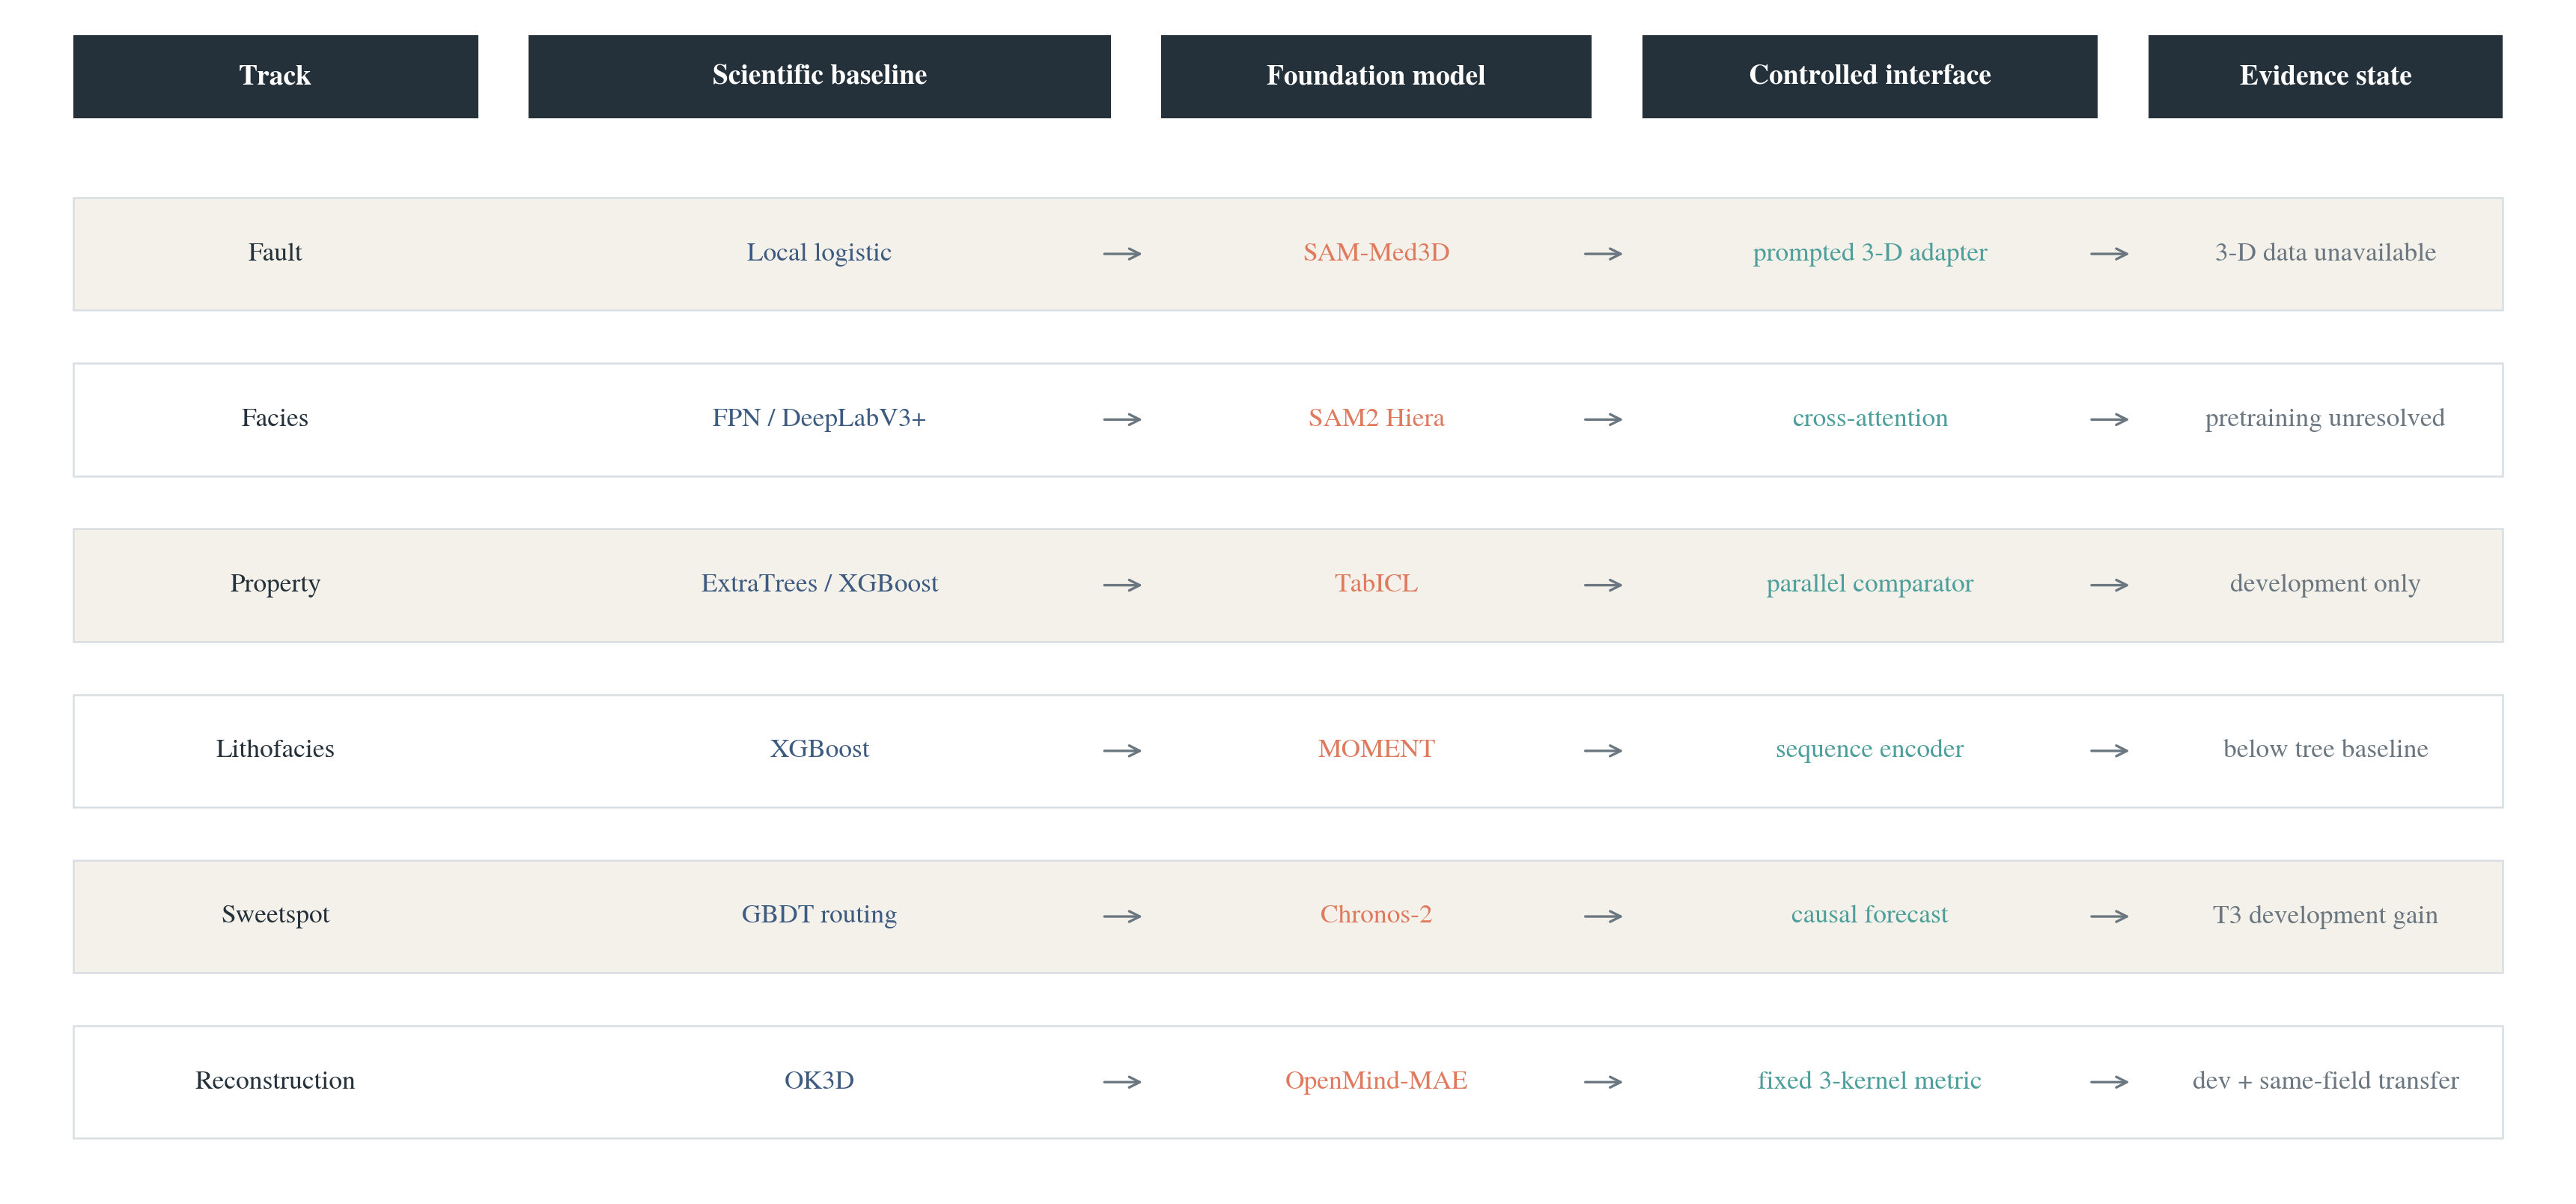
\includegraphics[width=0.98\textwidth]{../figures/results/foundation_model_research_map.png}
  \caption{六赛道基础模型研究设计。各赛道以强基线为参照，预训练模型分别通过独立
  对照、注意力融合、时序预测或邻域度量进入实验，并在固定划分下评价。}
  \label{fig:foundation-model-research-map}
\end{figure}

\section{实验原则}

所有赛道遵循三个原则。第一，数据划分先于模型训练确定，模型选择不得接触测试标签。
第二，主要评价指标在实验前固定，辅助指标只用于解释误差。第三，模型收益必须与
合理对照比较，包括强基线、历史均值、随机初始化或无基础模型分支。

对于已经被多次使用的留出集，本报告明确称为“已知留出集”，不把它包装成新的盲测。
对于没有合法开发折的任务，本报告只陈述基线结果，不推断候选模型已经胜出。这样的
表达可能更保守，但更接近实验事实。

\chapter{断层预测}

\section{任务背景}

断层预测的目标是从三维地震振幅体中识别不连续构造。输入为局部地震体
$\bm{X}\in\mathbb{R}^{H\times W\times D}$，输出为逐体素断层概率
$\bm{P}\in[0,1]^{H\times W\times D}$。断层通常只占很少的体素，类别极不平衡；
同时，断层面具有跨切片延续性，单张切片上的局部纹理不足以完整描述空间结构。

本赛道先建立可解释的局部逻辑回归基线，再评估 SAM-Med3D 的三维预训练表征
\cite{wang2023sammed3d}。研究问题不是简单判断“大模型是否更强”，而是检验三维
预训练表征能否在合法开发折上稳定改善断层分割。

\section{方法原理}

基线模型从地震振幅、局部梯度和不连续性响应中构造特征向量 $\bm{z}_i$，并用
逻辑函数估计第 $i$ 个体素属于断层的概率：
\begin{equation}
  p_i^{\mathrm{base}}=\sigma(\bm{w}^{\mathsf T}\bm{z}_i+b),
  \qquad
  \sigma(a)=\frac{1}{1+\exp(-a)} .
\end{equation}
其中 $\bm{w}$ 和 $b$ 分别为特征权重与截距。该模型参数少，便于检查局部特征与
断层概率之间的关系，适合作为小样本条件下的基线。

候选分支把三维地震块送入 SAM-Med3D 编码器，得到预训练特征
$\bm{h}_i^{\mathrm{sam}}$。适配头将其映射为候选概率 $p_i^{\mathrm{sam}}$，再由
门控系数 $g_i\in[0,1]$ 与基线融合：
\begin{equation}
  p_i=(1-g_i)p_i^{\mathrm{base}}+g_i p_i^{\mathrm{sam}} .
\end{equation}
当开发集证据不足时令 $g_i=0$，模型自动退回基线。这一设计把候选表征与默认预测
分开，避免未经验证的三维分支直接改变结果。

\ArchitectureFigure{fault}
  {断层预测模型架构。局部可解释基线与 SAM-Med3D 三维表征通过受控门融合。}
  {fault-architecture}

\Cref{fig:fault-architecture}描述目标模型的数据流。方法图中的三维分支能否进入
定量比较，仍取决于是否存在连续三维开发体。

\section{训练策略}

训练采用类别加权二元交叉熵。设正样本权重为 $\omega_1$，负样本权重为
$\omega_0$，则损失为
\begin{equation}
  \mathcal{L}_{\mathrm{WBCE}}
  =-\frac{1}{N}\sum_{i=1}^{N}
  \left[\omega_1 y_i\log p_i+\omega_0(1-y_i)\log(1-p_i)\right].
\end{equation}
权重由训练集类别频率确定，本次实验的负类与正类权重分别为 $0.5053$ 和
$47.7847$。模型训练 120 个 epoch，批量大小为 16，并根据验证集损失选择第 16
个 epoch 的参数。

概率阈值也只在验证集上选择。最终阈值为 $0.4506$，对应验证集 F1 的最大值。
测试集只在模型和阈值固定后评价一次。

\TrainingFlow
  {地震体与断层标签}
  {局部块采样}
  {加权损失训练}
  {验证集选模型}
  {固定阈值测试}
  {断层预测训练流程}
  {fault-training}

\section{实验设计}

基线实验使用 198 个训练样本、56 个验证样本和 96 个测试样本。现有样本是彼此独立
的二维剖面，输入通道形状为 $1\times33\times65$，输出为逐像素断层概率。理论任务
目标仍是三维体素预测；候选实验需要在连续三维数据上增加预训练编码器，并由独立
开发折评价。

进一步检查发现，当前三维赛道没有满足约束的合法开发折。因此，SAM-Med3D 分支
尚不能完成公平排名，冻结测试集也没有用于候选模型选择。本章报告的定量结果来自
已完成独立复核的基线；方法架构用于说明后续实验的比较对象。

\section{评估指标}

断层预测同时评价检出能力和空间重叠。精确率与召回率分别为
\begin{equation}
  \Metric{Precision}=\frac{TP}{TP+FP},
  \qquad
  \Metric{Recall}=\frac{TP}{TP+FN}.
\end{equation}
Dice 系数和交并比定义为
\begin{equation}
  \Metric{Dice}=\frac{2TP}{2TP+FP+FN},
  \qquad
  \Metric{IoU}=\frac{TP}{TP+FP+FN}.
\end{equation}
由于正类稀少，准确率会被大量背景体素主导，因此本赛道以 Dice、IoU、平均精确率
（AP）和 PR-AUC 为主要指标，并用召回率检查漏检风险。

\section{实验结果}

\begin{table}[htbp]
  \centering
  \caption{断层预测基线的测试结果}
  \label{tab:fault-results}
  \begin{tabular}{lrrrrr}
    \toprule
    模型 & Precision & Recall & Dice/F1 & IoU & AP \\
    \midrule
    局部逻辑回归 & 0.0078 & 0.9022 & 0.0155 & 0.0078 & 0.0069 \\
    \bottomrule
  \end{tabular}
\end{table}

\Cref{tab:fault-results}显示，基线取得 $0.9022$ 的召回率，但精确率只有
$0.0078$。这说明模型能够覆盖大部分
真实断层，却产生了大量误检。Dice 和 IoU 均较低，当前模型更适合作为高召回的
候选区域生成器，尚不足以直接承担精确断层制图。

\ResultFigure{0.92}{fault}{research_geological_context.png}
  {Volve 断层棒与 BCU 层位在真实 UTM--TWT 坐标中的空间关系。该图展示解释几何，
  不把稀疏断层棒扩展为未验证的连续概率体。}

\ResultFigure{0.94}{fault}{research_seismic_overlay.png}
  {Inline 10243 的原始地震剖面与同一剖面上的断层解释控制点。连线仅连接同一断层棒
  中至少两个控制点，用于核对解释位置与反射不连续结构。}

三维场景说明断层解释并不是无坐标的样本集合，而是位于已配准地震网格中的空间
结构。剖面核对进一步显示，进入连线的控制点主要分布在反射同相轴发生弯折或中断的
区域。两幅图只验证解释与地震背景的几何一致性，不能替代模型的体素级预测评价。

\ResultPair{fault}
  {real_test_panel.png}{测试样本上的输入、标签与预测}
  {spatial_context.png}{断层预测的空间位置与邻域结构}
  {断层预测的样本级与空间级结果}

\ResultPair{fault}
  {loss_curve.png}{训练与验证损失}
  {prediction_visualization.png}{概率预测与二值结果}
  {基线模型的优化过程与预测表现}

当前实验的主要问题是误检，而不是漏检。后续实验应先补齐合法三维
开发折，再比较局部基线、随机初始化三维编码器和 SAM-Med3D 三组模型；只有当预训练
分支在独立开发折上稳定提高 Dice、PR-AUC 和表面距离指标时，才有理由进入最终预测。

\FloatBarrier

\chapter{地震相分割}

\section{任务背景}

地震相分割根据多道地震切片识别不同沉积或构造相。输入为三通道地震切片
$\bm{X}\in\mathbb{R}^{3\times H\times W}$，输出为每个像素的类别概率。
F3 和 Penobscot 的相类别数、纹理与信噪比不同，因此分别使用
FPN--ResNet18 和 DeepLabV3+--ResNet18 作为卷积基线。

\section{方法原理}

卷积主干输出语义特征 $\bm{F}_{\mathrm{cnn}}$，SAM2 编码器
\cite{ravi2024sam2} 从同一切片提取预训练特征 $\bm{F}_{\mathrm{sam}}$。
交叉注意力以卷积特征为查询、SAM2 特征为键和值：
\begin{align}
  \bm{Q}&=\bm{W}_Q\bm{F}_{\mathrm{cnn}},&
  \bm{K}&=\bm{W}_K\bm{F}_{\mathrm{sam}},&
  \bm{V}&=\bm{W}_V\bm{F}_{\mathrm{sam}},\\
  \bm{A}&=\mathrm{softmax}\!\left(
    \frac{\bm{Q}\bm{K}^{\mathsf T}}{\sqrt{d}}
  \right)\bm{V}.
\end{align}
其中 $\bm{W}_Q,\bm{W}_K,\bm{W}_V$ 为线性投影矩阵，$d=128$，注意力头数为 4。
融合特征为
\begin{equation}
  \bm{F}_{\mathrm{fused}}
  =\bm{F}_{\mathrm{cnn}}+\gamma\bm{W}_O\bm{A},
\end{equation}
其中 $\gamma$ 为可学习系数。\Cref{fig:facies-architecture}给出了完整的数据流。

\ArchitectureFigure{facies}
  {地震相分割模型架构。卷积语义特征查询 SAM2 表征，经交叉注意力融合后送入解码器。}
  {facies-architecture}

\section{训练策略}

训练目标由像素交叉熵与软 Dice 损失组成：
\begin{equation}
  \mathcal{L}=\mathcal{L}_{\mathrm{CE}}+
  0.25\,\mathcal{L}_{\mathrm{Dice}} .
\end{equation}
训练集使用水平翻转和高斯噪声增强，验证集不做增强。卷积主干学习率为
$5\times10^{-5}$，融合层学习率为 $2\times10^{-4}$，SAM2 可训练块学习率为
$10^{-5}$；优化过程采用余弦退火。

\TrainingFlow
  {三通道地震切片}
  {固定空间折}
  {训练集增强}
  {卷积与 SAM2 编码}
  {交叉注意力与解码}
  {地震相分割训练流程}
  {facies-training}

\section{实验设计}

F3 使用第 0 折，Penobscot 使用第 4 折。每个数据集比较三种模型：40 次更新的强卷积
基线、160 次更新的继续训练卷积对照，以及 160 次更新的 SAM2 交叉注意力模型。
SAM2 加载真实预训练权重，仅解冻 Hiera 的第 22 和 23 个块。每次实验最多使用
32 个训练样本和 16 个验证样本，批量大小为 2。实验只访问固定开发折，不读取冻结
测试集。三臂设计用于区分额外训练预算与交叉注意力分支的作用。

\section{评估指标}

主要指标为平均交并比：
\begin{equation}
  \Metric{mIoU}=\frac{1}{C}\sum_{c=1}^{C}
  \frac{TP_c}{TP_c+FP_c+FN_c}.
\end{equation}
其中 $TP_c$、$FP_c$ 和 $FN_c$ 分别为第 $c$ 类的真阳性、假阳性和假阴性像素数。
同时报告像素准确率、Macro-F1 和负对数似然，以描述分类性能与概率质量。

\section{实验结果}

\begin{table}[htbp]
  \centering
  \caption{地震相分割的固定开发折结果}
  \label{tab:facies-dev}
  \begin{tabular}{llrr}
    \toprule
    数据集 & 模型 & mIoU & Macro-F1 \\
    \midrule
    F3 & 40 次更新卷积基线 & 0.1363 & 0.2215 \\
    F3 & 160 次更新卷积对照 & 0.2069 & 0.3145 \\
    F3 & SAM2 交叉注意力 & \textbf{0.2922} & \textbf{0.4164} \\
    \midrule
    Penobscot & 40 次更新卷积基线 & 0.1291 & 0.1766 \\
    Penobscot & 160 次更新卷积对照 & 0.1896 & 0.2624 \\
    Penobscot & SAM2 交叉注意力 & \textbf{0.2053} & \textbf{0.2826} \\
    \bottomrule
  \end{tabular}
\end{table}

\Cref{tab:facies-dev}显示，两个数据集的平均 mIoU 从 $0.1327$ 提高到 $0.2487$，
绝对增益为 $0.1160$。与继续训练卷积对照相比，F3 和 Penobscot 分别提高
$0.0853$ 和 $0.0157$，说明额外训练预算不能完全解释结果。

\ResultFigure{0.98}{facies}{research_f3_curtains.png}
  {F3 连续地震体中三个已配准 inline 切面的振幅与十类解释。左侧为原始地震振幅，
  右侧为同位置参考类别；两者均为数据证据，不是当前 SAM2 模型的稠密预测。}

\Cref{fig:res-facies-research_f3_curtains.png}把二维样本放回连续三维索引中。三个
切面同时保留 inline、crossline 和采样点坐标，因此可以检查相带沿空间方向的延续性。
当前归档结果没有保存 SAM2 的完整三维概率体，故本版不构造预测混淆矩阵或相体表面；
这些图必须在稠密预测落盘后才能进入模型结果。

\ResultPair{facies}
  {facies_f3_stage3_oof_diagnostics.png}{F3 既有基线的折外诊断}
  {facies_penobscot_stage3_oof_diagnostics.png}{Penobscot 既有基线的折外诊断}
  {两个数据集的既有基线诊断}

\ResultPair{facies}
  {f3_known_holdout_diagnostics.png}{F3 历史留出诊断}
  {penobscot_known_holdout_diagnostics.png}{Penobscot 历史留出诊断}
  {既有模型在历史留出数据上的诊断}

\Cref{tab:facies-dev}与历史留出诊断并非同一次模型评价。前者是本次
SAM2 交叉注意力的固定开发折结果，后者仅说明既有分割流程的误差形态，不能据此宣称
SAM2 已在留出集上获得同等增益。此外，同结构随机初始化 SAM2 分支尚未完成，因此
当前结论应表述为“交叉注意力系统在开发集上更优”，而非“预训练权重已经被证明有效”。

\FloatBarrier

\chapter{储层物性预测}

\section{任务背景}

储层物性预测根据井曲线和地质位置估计孔隙度、渗透率与含水饱和度。本赛道包含三个
连续目标：孔隙度 PHIF、水平渗透率 KLOGH 和含水饱和度 SW。输入为同深度位置的
多条测井曲线及派生特征，输出为目标物性的点估计和不确定性区间。

三类物性的统计分布不同。PHIF 与 SW 的数值范围相对集中，KLOGH 则具有明显长尾，
可跨越多个数量级。因此，本赛道不强行使用同一回归器，而是根据目标分布选择模型，
再用统一的留出评价比较结果。

\section{方法原理}

PHIF 和 KLOGH 使用极端随机树。设第 $m$ 棵树的预测为 $f_m(\bm{x})$，集成输出为
\begin{equation}
  \hat{y}=\frac{1}{M}\sum_{m=1}^{M}f_m(\bm{x}).
\end{equation}
随机特征和随机切分降低了单棵树的方差，适合处理非线性井曲线关系。KLOGH 在
$\log(1+y)$ 域训练，以减弱长尾样本对平方误差的支配。

SW 使用 XGBoost。第 $t$ 轮在已有预测上增加一棵回归树：
\begin{equation}
  \hat{y}^{(t)}_i=\hat{y}^{(t-1)}_i+\eta f_t(\bm{x}_i),
\end{equation}
其中 $\eta$ 为学习率。候选基础模型 TabICL 通过上下文学习读取表格样本
\cite{qu2025tabicl}，其输出作为独立对照分支，不直接覆盖树模型结果。

预测区间由训练折外残差构造。若绝对残差的 $90\%$ 分位数为 $q_{0.9}$，则区间写为
\begin{equation}
  [\hat{y}-q_{0.9},\ \hat{y}+q_{0.9}] .
\end{equation}
该区间不假设残差服从正态分布，更适合分布偏斜的物性变量。

\ArchitectureFigure{property}
  {储层物性预测模型架构。三个目标使用与其分布相匹配的树模型，并由折外残差给出预测区间。}
  {property-architecture}

\section{训练策略}

数据按井族划分，避免同一口井的相邻深度同时出现在训练集和评价集。缺失值处理、
特征缩放和目标变换只在训练数据上拟合，再应用到验证和留出数据。模型参数通过开发
折选择，最终参数固定后在已知留出井族 15/9-F-15 上评价。

PHIF 与 KLOGH 的树数量、叶节点样本数和特征采样率通过交叉验证确定；SW 进一步
优化树深、学习率和迭代轮数。TabICL 使用相同输入与划分，比较真实预训练权重与
传统树模型；后续还需加入同架构随机权重对照，才能判断收益是否来自预训练。

\TrainingFlow
  {井曲线与深度}
  {按井族划分}
  {目标变换与特征处理}
  {树模型参数优化}
  {留出集与区间评价}
  {储层物性预测训练流程}
  {property-training}

\section{实验设计}

实验分别训练 PHIF、KLOGH 和 SW 三个模型。输入包括原始井曲线、邻域统计和空间
位置，输出包括点预测、残差和 $90\%$ 预测区间。主要对照为每个目标的赛道基线，
基础模型分支只用于检查表格预训练表征是否提供额外信息。

留出集共有 344 个有效样本。该井族在历史实验中已经使用，因此本章将其称为已知
留出集，而不称为全新盲测。实验重点是确认当前模型在固定数据口径下能否复现，而非
用同一留出集继续选择模型。

\section{评估指标}

连续变量使用决定系数、均方根误差、平均绝对误差和偏差：
\begin{align}
  R^2 &= 1-\frac{\sum_i(y_i-\hat{y}_i)^2}
  {\sum_i(y_i-\bar{y})^2},\\
  \Metric{RMSE} &= \sqrt{\frac{1}{N}\sum_i(y_i-\hat{y}_i)^2},\\
  \Metric{MAE} &= \frac{1}{N}\sum_i|y_i-\hat{y}_i|,\\
  \Metric{Bias} &= \frac{1}{N}\sum_i(\hat{y}_i-y_i).
\end{align}
预测区间还评价覆盖率，即真实值落入区间的比例，以及平均区间宽度。理想区间应在
接近目标覆盖率的同时保持较窄；仅追求高覆盖率会得到缺乏信息的宽区间。

\section{实验结果}

\begin{table}[htbp]
  \centering
  \caption{三类物性在已知留出集上的结果}
  \label{tab:property-holdout}
  \begin{tabular}{llrrrrr}
    \toprule
    目标 & 模型 & $R^2$ & RMSE & MAE & Bias & 覆盖率 \\
    \midrule
    PHIF & ExtraTrees & 0.9807 & 0.0093 & 0.0061 & 0.0006 & 0.9942 \\
    KLOGH & ExtraTrees & 0.8891 & 278.8388 & 145.6398 & 71.2485 & 1.0000 \\
    SW & XGBoost & 0.9032 & 0.0806 & 0.0644 & 0.0240 & 0.9942 \\
    \bottomrule
  \end{tabular}
\end{table}

\Cref{tab:property-holdout}显示，PHIF 的 $R^2$ 达到 $0.9807$，点预测误差较小。
SW 的 $R^2$ 为 $0.9032$，仍存在
轻微正偏。KLOGH 在物理域的 $R^2$ 为 $0.8891$，但 RMSE 达到
$278.84\,\mathrm{mD}$；在 $\log(1+y)$ 训练域中，其 $R^2$ 为 $0.9130$。这说明
模型能够解释总体变化，但极高渗透率样本仍主导物理域误差。

\begin{table}[htbp]
  \centering
  \caption{TabICL 与树模型在开发折上的初步比较}
  \label{tab:property-tabicl}
  \begin{tabular}{lrrr}
    \toprule
    目标 & 树模型 RMSE & TabICL RMSE & 相对变化 \\
    \midrule
    PHIF & 0.02764 & 0.02629 & $-4.89\%$ \\
    KLOGH & 542.9026 & 469.2547 & $-13.57\%$ \\
    SW & 0.17043 & 0.12750 & $-25.19\%$ \\
    \bottomrule
  \end{tabular}
\end{table}

\Cref{tab:property-tabicl}仅报告开发折机制实验。TabICL 在三个目标上均降低 RMSE，
且优于目标置乱对照，但同架构随机初始化对照尚未完成。因此，这些结果不能替代
\Cref{tab:property-holdout}中的已知留出结果，也不能单独证明增益来自预训练权重。

\ResultFigure{0.92}{property}{phif_heldout_summary.png}
  {PHIF 在已知留出集上的预测、残差与区间诊断。}

\ResultFigure{0.92}{property}{klogh_heldout_summary.png}
  {KLOGH 在已知留出集上的预测、残差与区间诊断。横轴变换仅用于展示长尾分布。}

\ResultFigure{0.92}{property}{sw_heldout_summary.png}
  {SW 在已知留出集上的预测、残差与区间诊断。}

\ResultPair{property}
  {before_after_primary_metric.png}{主要指标的阶段比较}
  {loss_curve.png}{模型优化过程}
  {储层物性预测的整体比较与训练表现}

\ResultFigure{0.98}{property}{research_well_diagnostics.png}
  {同一已知留出井段上的 PHIF、KLOGH 与 SW 观测、预测、经验残差区间及逐深度残差。
  KLOGH 保留物理单位并采用对数坐标显示。}

\ResultFigure{0.92}{property}{research_rock_physics_crossplot.png}
  {相同留出样本上的 PHIF--KLOGH 联合关系。左图为观测，右图为两个独立回归器的
  预测，颜色表示测量深度。}

单目标指标不能判断多个物性预测是否仍然满足一致的岩石物理关系。观测样本中 PHIF
与 $\log(1+\mathrm{KLOGH})$ 的 Pearson 相关系数为 $0.704$，独立预测后的相关系数
为 $0.790$。模型保留了总体正相关，但提高的相关强度也提示预测可能压缩局部离散度；
因此，联合关系应作为物理一致性诊断，而不能替代三个目标各自的留出误差。

三个目标的区间覆盖率均高于 $0.99$，但 KLOGH 的平均区间宽度达到
$2879.75\,\mathrm{mD}$。因此，高覆盖率并不表示不确定性已经解决。下一步应针对
KLOGH 的长尾区间进行分层校准，并补充新的井族盲测。

\FloatBarrier

\chapter{岩相分类}

\section{任务背景}

岩相分类根据井曲线序列判断每个深度点所属的地质相。本赛道固定使用 9 类遗传岩相，
即使某个评价井不包含其中部分类型，评价时也保留完整类别集合。输入为目标深度附近的
多道测井窗口，输出为 9 类概率和最终类别。

该任务同时具有表格与序列特征。单个深度点的曲线值提供局部物性信息，邻近深度的
变化趋势则反映层序结构。小样本、类别不平衡和跨井分布差异是主要困难。

\section{方法原理}

主模型使用 XGBoost 多类 softprob。对第 $c$ 类，模型累加多棵树得到得分
$s_c(\bm{x})$，再用 softmax 转换为概率：
\begin{equation}
  p(y=c\mid\bm{x})
  =\frac{\exp(s_c(\bm{x}))}{\sum_{k=1}^{9}\exp(s_k(\bm{x}))}.
\end{equation}
输入特征由中心深度的测井值、窗口统计量和局部变化率组成。树模型能够处理非线性
特征交互，也能在样本量有限时保持较低方差。

候选分支使用 MOMENT-1-base 对多通道深度窗口进行分类
\cite{goswami2024moment}。设窗口为 $\bm{X}$，冻结编码器输出为
$\bm{e}=E_{\theta}(\bm{X})$，九类线性头写为
\begin{equation}
  \bm{p}=\mathrm{softmax}(\bm{W}\bm{e}+\bm{b}).
\end{equation}
输入包含 35 个通道和 33 个深度位置，编码器内部插值到长度 512。预训练 MOMENT
与同架构随机初始化 MOMENT 使用相同的九类分类头，因而可直接检验预训练权重的作用。

\ArchitectureFigure{lithofacies}
  {岩相分类模型架构。井曲线窗口同时进入树模型与 MOMENT 序列表征分支。}
  {lithofacies-architecture}

\section{训练策略}

数据按母井执行四折留一井交叉验证（LOGO4）。每一折以三口井训练，剩余一口井验证，
确保相邻深度样本不会跨越训练和验证边界。窗口归一化、缺失值填补和类别权重均只由
当折训练井计算。

模型选择以固定 9 类 Macro-F1 为主，而不是只对当前验证井中出现的类别求平均。
对每个候选参数组合重复多个随机种子，并观察折间方差。最终模型固定后，再在已知
留出井族 15/9-F-5 上做确认性评价。

\TrainingFlow
  {九类井曲线标签}
  {按母井 LOGO4}
  {窗口特征与归一化}
  {多种子模型训练}
  {固定九类评价}
  {岩相分类训练流程}
  {lithofacies-training}

\section{实验设计}

实验比较三种分类器：固定九类 XGBoost、真实预训练权重的 MOMENT，以及同架构
随机初始化 MOMENT。三者使用相同的 LOGO4 开发折。缺失模态实验进一步移除部分
曲线，用于检查模型对真实测井缺失的敏感性。

开发阶段用 LOGO4 选择参数，确认阶段使用 120 个已知留出样本。部分岩相在该井族中
没有支持样本，因此同时报告固定 9 类指标和“仅对有支持类别求平均”的诊断指标。
后者帮助解释当前井的表现，但不替代主要指标。

\section{评估指标}

主要指标为固定 9 类 Macro-F1：
\begin{equation}
  \Metric{MacroF1}_{9}
  =\frac{1}{9}\sum_{c=1}^{9}
  \frac{2TP_c}{2TP_c+FP_c+FN_c}.
\end{equation}
此外报告固定 9 类平均交并比、准确率和概率质量。多类负对数似然与 Brier 分数分别为
\begin{align}
  \Metric{NLL} &=-\frac{1}{N}\sum_{i=1}^{N}\log p_{i,y_i},\\
  \Metric{Brier} &=\frac{1}{N}\sum_{i=1}^{N}
  \sum_{c=1}^{9}\left(p_{ic}-\mathbb{I}(y_i=c)\right)^2.
\end{align}
期望校准误差（ECE）比较概率置信度与实际正确率，用于判断模型是否过度自信。

\section{实验结果}

\begin{table}[htbp]
  \centering
  \caption{岩相分类在已知留出井族上的结果}
  \label{tab:litho-holdout}
  \begin{tabular}{lr}
    \toprule
    指标 & 数值 \\
    \midrule
    Accuracy & 0.4167 \\
    固定 9 类 Macro-F1 & 0.1892 \\
    有支持类别 Macro-F1（诊断） & 0.2432 \\
    固定 9 类 mIoU & 0.1288 \\
    NLL & 1.7022 \\
    Multiclass Brier & 0.7938 \\
    ECE & 0.1415 \\
    \bottomrule
  \end{tabular}
\end{table}

\Cref{tab:litho-holdout}中的固定 9 类 Macro-F1 为 $0.1892$，与开发阶段
XGBoost 的 $0.1949$ 接近，说明当前
流程可以复现，但总体分类能力仍有限。准确率为 $0.4167$，明显高于 Macro-F1，
说明结果受多数类主导。ECE 为 $0.1415$，概率仍有进一步校准空间。

\begin{table}[htbp]
  \centering
  \caption{岩相分类在 LOGO4 开发折上的模型比较}
  \label{tab:litho-dev}
  \begin{tabular}{lr}
    \toprule
    模型 & 固定 9 类 Macro-F1 \\
    \midrule
    XGBoost & \textbf{0.1949} \\
    MOMENT 真实预训练权重 & 0.0463 \\
    MOMENT 同架构随机初始化 & 0.0411 \\
    \bottomrule
  \end{tabular}
\end{table}

\Cref{tab:litho-dev}表明，MOMENT 真实权重略优于随机初始化，说明预训练表征包含
少量可迁移信息；但其 Macro-F1 远低于 XGBoost。因此，MOMENT 不应替代当前树模型。

\ResultFigure{0.94}{lithofacies}{before_after_primary_metric.png}
  {岩相分类主要指标的阶段比较。}

\ResultPair{lithofacies}
  {fixed9_confusion.png}{固定九类混淆矩阵}
  {fixed9_per_class_pr_f1_support.png}{类别级精确率、召回率与支持度}
  {固定九类条件下的分类结构}

\ResultPair{lithofacies}
  {calibration_reliability.png}{概率校准曲线}
  {missing_modality_diagnostic.png}{缺失测井模态诊断}
  {预测置信度与输入完整性分析}

\ResultPair{lithofacies}
  {fold_seed_matrix.png}{跨井折与随机种子的稳定性}
  {multimodal_mlp_loss_curve.png}{多模态 MLP 的训练过程}
  {岩相分类的稳定性与优化过程}

\ResultFigure{0.94}{lithofacies}{research_well_sequence.png}
  {已知留出井 15/9-F-5 的固定九类观测序列、XGBoost 预测序列和逐样本最大类别概率。
  纵轴采用归档记录中的 TWT；红点表示误分类位置。}

\Cref{fig:res-lithofacies-research_well_sequence.png}显示，错误样本与正确样本的平均
最大类别概率分别为 $0.506$ 和 $0.501$，两者几乎没有分离。这说明当前置信度不能
有效识别错误区间，与 ECE 仍偏高的结果一致。由于归档预测未包含经过核验的井轨迹
XYZ 坐标，本章只报告 TWT 序列，不把一维井段外推为三维岩相体。

同架构随机初始化对照已经完成，结论不是“仍待归因”，而是“存在轻微预训练效应，
但不足以超过强基线”。后续工作的重点应是扩大母井样本、改善少数类学习和检验
跨井泛化，而不是继续提高 MOMENT 分类头的训练预算。

\FloatBarrier

\chapter{甜点评价}

\section{任务背景}

甜点评价把地质、储层和生产信息分解为七个具有独立定义的目标。T1 是储层质量指数
代理量 $0.0314\sqrt{\mathrm{KLOGH}/\mathrm{PHIF}}$；T2 是近二元的砂岩标志代理；
T3 是预测时点后 30 个日历日内、至少 24 个有效观测日的平均产油量；T4 是未来
30 日内连续 7 个有效日出现产水的代理标签。T1、T2 和 T4 不是现场甜点真值，
只有 T3 属于观测生产结果。

T5 表示剩余油或加密井潜力，但尚无经审定的标签；T6 和 T7 分别对应解释得到的 PHIF
与 KLOGH，其多模态生产路径尚缺可迁移的开发期地震特征。不同目标的数据量和时间
结构差异很大，因此本赛道按目标选择模型，并分别报告结果。

\section{方法原理}

T1 使用 LightGBM，T2 与 T4 使用 CatBoost。两类提升树都以加法模型逐步拟合残差，
一般形式为
\begin{equation}
  F_t(\bm{x})=F_{t-1}(\bm{x})+\eta f_t(\bm{x}),
\end{equation}
其中 $f_t$ 为第 $t$ 棵树，$\eta$ 为学习率。CatBoost 的有序目标统计有助于降低
类别特征中的目标泄漏。

T3 的主模型为 Chronos-2\cite{ansari2025chronos2}。模型读取目标历史、协变量和
预测时间点，输出未来生产量。为降低短序列上的波动，最终预测与训练期均值进行加权：
\begin{equation}
  \hat{y}_{T3}
  =\alpha\hat{y}_{\mathrm{Chronos2}}
  +(1-\alpha)\bar{y}_{\mathrm{train}},
\end{equation}
其中 $\alpha$ 只在当前训练折内部选择。MOMENT 用于时序表征对照，但不替代已经
通过开发集选择的 T3 路径。

\ArchitectureFigure{sweetspot}
  {甜点评价模型架构。七个目标分别建模，T3 由 Chronos-2 与训练期均值受控融合。}
  {sweetspot-architecture}

\section{训练策略}

静态任务按分组折划分，保证同一井或同一实体不会同时进入训练和验证。时序任务使用
滚动起点验证：每一折只用预测时刻之前的历史训练，并在随后的时间窗验证。T3 每折
最多使用 1024 个训练样本和 512 个验证样本，以固定计算规模。

T3 的融合权重 $\alpha$ 在折内训练数据上选择，再应用于该折验证窗口。候选模型按
平均绝对误差排序。T4 属于类别不平衡任务，因此按平均精确率选择，而不是按准确率
选择。T5--T7 在数据或任务定义不足时不训练占位模型。

\TrainingFlow
  {七项目标与协变量}
  {分组或滚动划分}
  {目标专属模型训练}
  {折内参数选择}
  {逐目标独立评价}
  {甜点评价训练流程}
  {sweetspot-training}

\section{实验设计}

T1 和 T2 的输入为静态井曲线，输出分别为 RQI 代理量与砂岩标志。T3 的输入为截止
$t_0$ 的产油、产气、产水、开井时长、井底压力、节流阀与井口压力序列，输出
$t_0+1$ 至 $t_0+30$ 日的平均产油量。T4 使用同类历史序列预测 30 日产水事件。
不完整时间窗作删失处理，不把缺测日填成零。

T3 同时比较三个基准：训练历史均值、归档 XGBoost 和 Chronos-2 融合。T4 比较
CatBoost 与 Chronos 候选分支。开发样本量分别为 T1 35810、T2 36122、T3 1111
和 T4 32；已知留出样本量分别为 11936、12081、132 和 37。T5 当前不可行，
T6 与 T7 仍受输入数据限制。

\section{评估指标}

回归任务使用 MAE、RMSE 和 $R^2$。其中
\begin{equation}
  \Metric{MAE}=\frac{1}{N}\sum_i|y_i-\hat{y}_i|,
  \qquad
  \Metric{RMSE}=\sqrt{\frac{1}{N}\sum_i(y_i-\hat{y}_i)^2}.
\end{equation}
分类任务使用平均精确率、Macro-F1 和 ROC-AUC。平均精确率对精确率--召回率曲线
进行加权求和：
\begin{equation}
  \Metric{AP}=\sum_n(R_n-R_{n-1})P_n,
\end{equation}
其中 $P_n$ 和 $R_n$ 分别为第 $n$ 个阈值下的精确率和召回率。每个目标独立评价，
不把不同单位的指标相加为综合分数。

\section{实验结果}

\begin{table}[htbp]
  \centering
  \caption{T3 时序预测的滚动验证结果}
  \label{tab:sweetspot-t3-dev}
  \begin{tabular}{lrr}
    \toprule
    模型 & MAE & 相对 Chronos-2 的 MAE 增幅 \\
    \midrule
    归档 XGBoost & 267.1180 & $+43.17\%$ \\
    因果历史均值 & 204.6371 & $+9.68\%$ \\
    Chronos-2 融合 & \textbf{186.5715} & -- \\
    \bottomrule
  \end{tabular}
\end{table}

\Cref{tab:sweetspot-t3-dev}显示，Chronos-2 融合的 MAE 为 $186.57$，相对归档
XGBoost 降低 $30.15\%$，相对
因果历史均值降低 $8.83\%$，满足预设的开发集改进标准。T4 中，Chronos 分支的
AP 为 $0.5091$，低于 CatBoost 的 $0.6541$，因此未达到改进标准。两项结果说明同一基础模型
在不同目标上可能产生相反结论，必须逐任务评价。

\begin{table}[htbp]
  \centering
  \caption{四个可评价目标的已知留出结果}
  \label{tab:sweetspot-holdout}
  \small
  \begin{tabular}{llllr}
    \toprule
    目标 & 留出模型 & 主要指标 & 辅助指标 & 样本量 \\
    \midrule
    T1 & LightGBM & $R^2=0.8968$ & MAE $=0.2162$ & 11936 \\
    T2 & CatBoost & AP $=0.9991$ & F1 $=0.9777$ & 12081 \\
    T3 & 归档 XGBoost & MAE $=47.7020$ & $R^2=-0.0636$ & 132 \\
    T4 & CatBoost & AP $=0.1315$ & F1 $=0.1951$ & 37 \\
    \bottomrule
  \end{tabular}
\end{table}

\Cref{tab:sweetspot-holdout}报告的是早期阶段固定模型在已知留出集上的确认结果，
不能解释为 Chronos-2 的留出表现。尤其是 T4 的开发 AP 为 $0.6541$，已知留出
AP 仅为 $0.1315$；结合留出样本量只有 37，这一差异提示小样本波动和分布偏移风险。

\ResultFigure{0.98}{sweetspot}{research_target_diagnostics.png}
  {T1 储层质量代理的逐深度观测、预测与残差，以及 T3 生产率在因果时间轴上的观测、
  预测与残差。两个目标保持独立单位，不合成为单一评分。}

\ResultFigure{0.92}{sweetspot}{research_productivity_performance.png}
  {T3 已知留出集的实测--预测散点与标准化残差 Q--Q 图。散点按预测时序着色，
  虚线分别表示理想预测和正态残差参照。}

T3 的确认模型在已知留出集上取得 $R^2=-0.0636$，实测--预测散点仍明显偏离
单位线。残差 Q--Q 图在两端偏离参照线，说明极端生产阶段的误差不能由简单正态扰动
解释。该结果与开发阶段的 Chronos-2 改进并不矛盾：两者对应不同模型和证据阶段，
真正的下一步是对 Chronos-2 完成同口径时序留出评价，而不是用开发增益替代留出结论。

\ResultFigure{0.96}{sweetspot}{overview_seven_targets.png}
  {甜点评价七个目标的定义、数据可用性与主要结果总览。}

\ResultPair{sweetspot}
  {T1_regression_diagnostics.png}{T1 回归诊断}
  {T2_classification_diagnostics.png}{T2 分类诊断}
  {T1 与 T2 的实验结果}

\ResultPair{sweetspot}
  {T3_regression_diagnostics.png}{T3 时序回归诊断}
  {T4_classification_diagnostics.png}{T4 分类诊断}
  {T3 与 T4 的实验结果}

\begin{figure}[htbp]
  \centering
  \begin{subfigure}[t]{0.32\textwidth}
    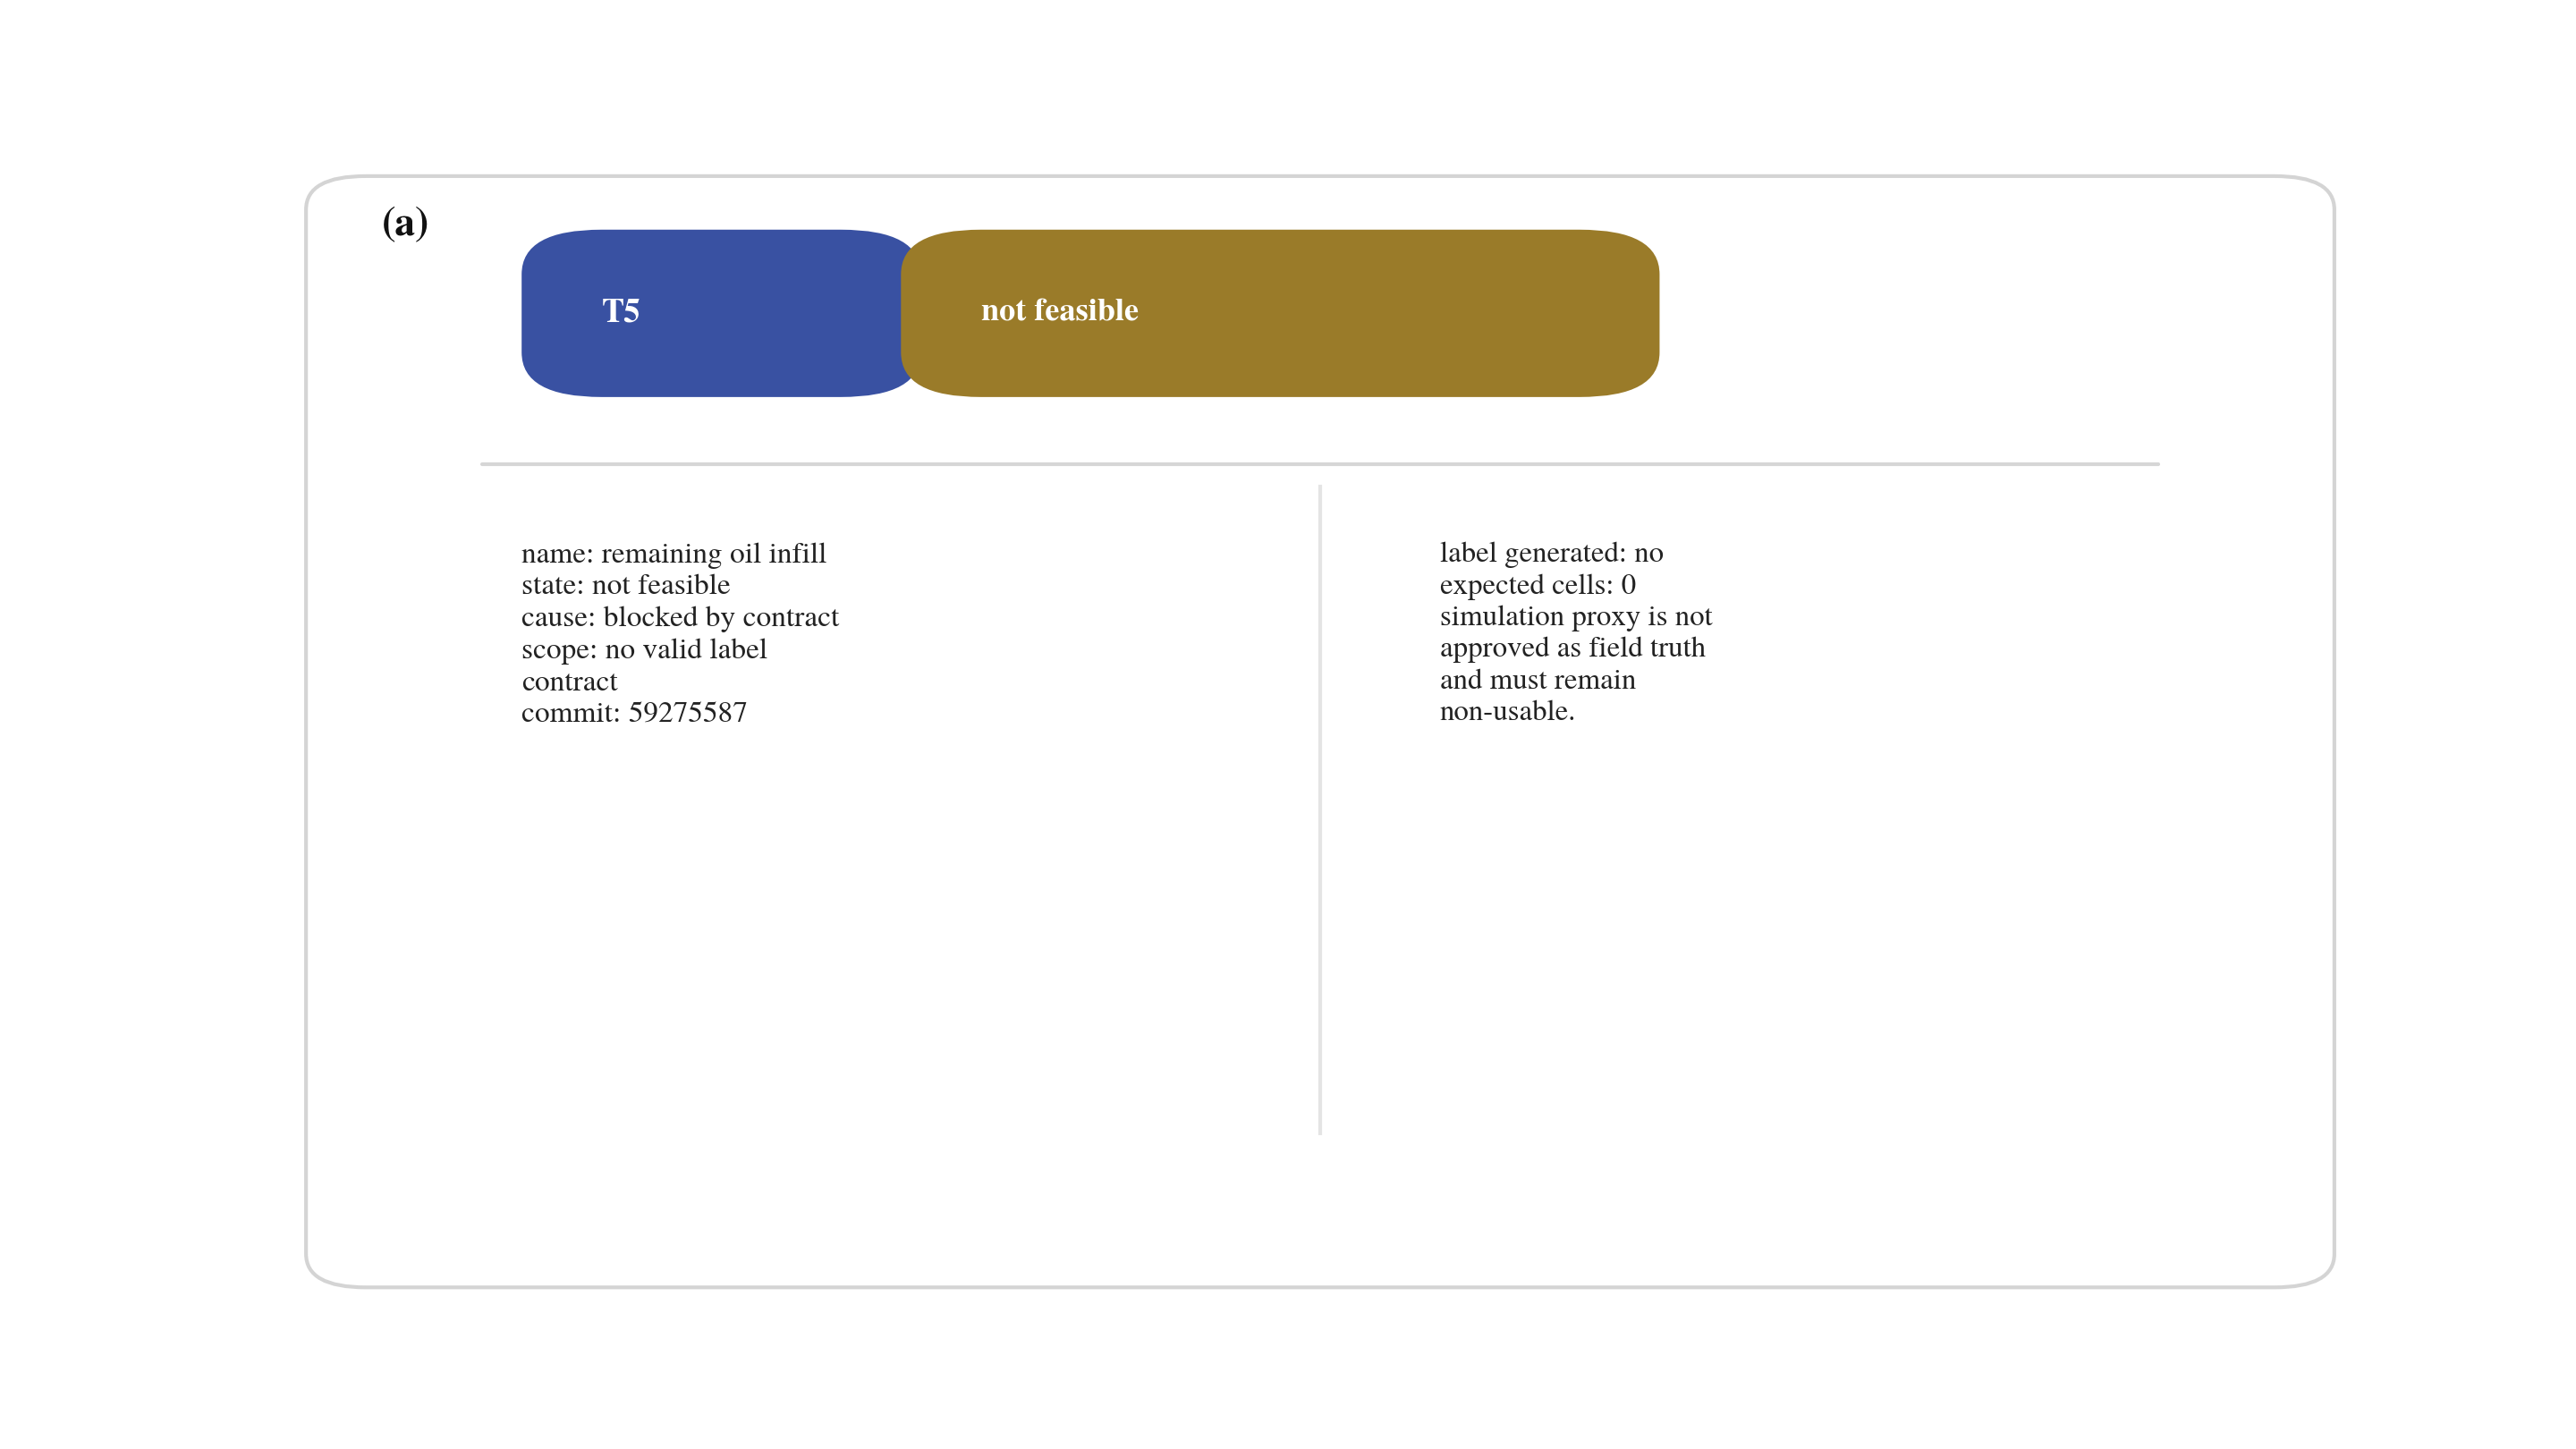
\includegraphics[width=\textwidth]{../figures/results/sweetspot/T5_status_card.png}
    \caption{T5}
  \end{subfigure}\hfill
  \begin{subfigure}[t]{0.32\textwidth}
    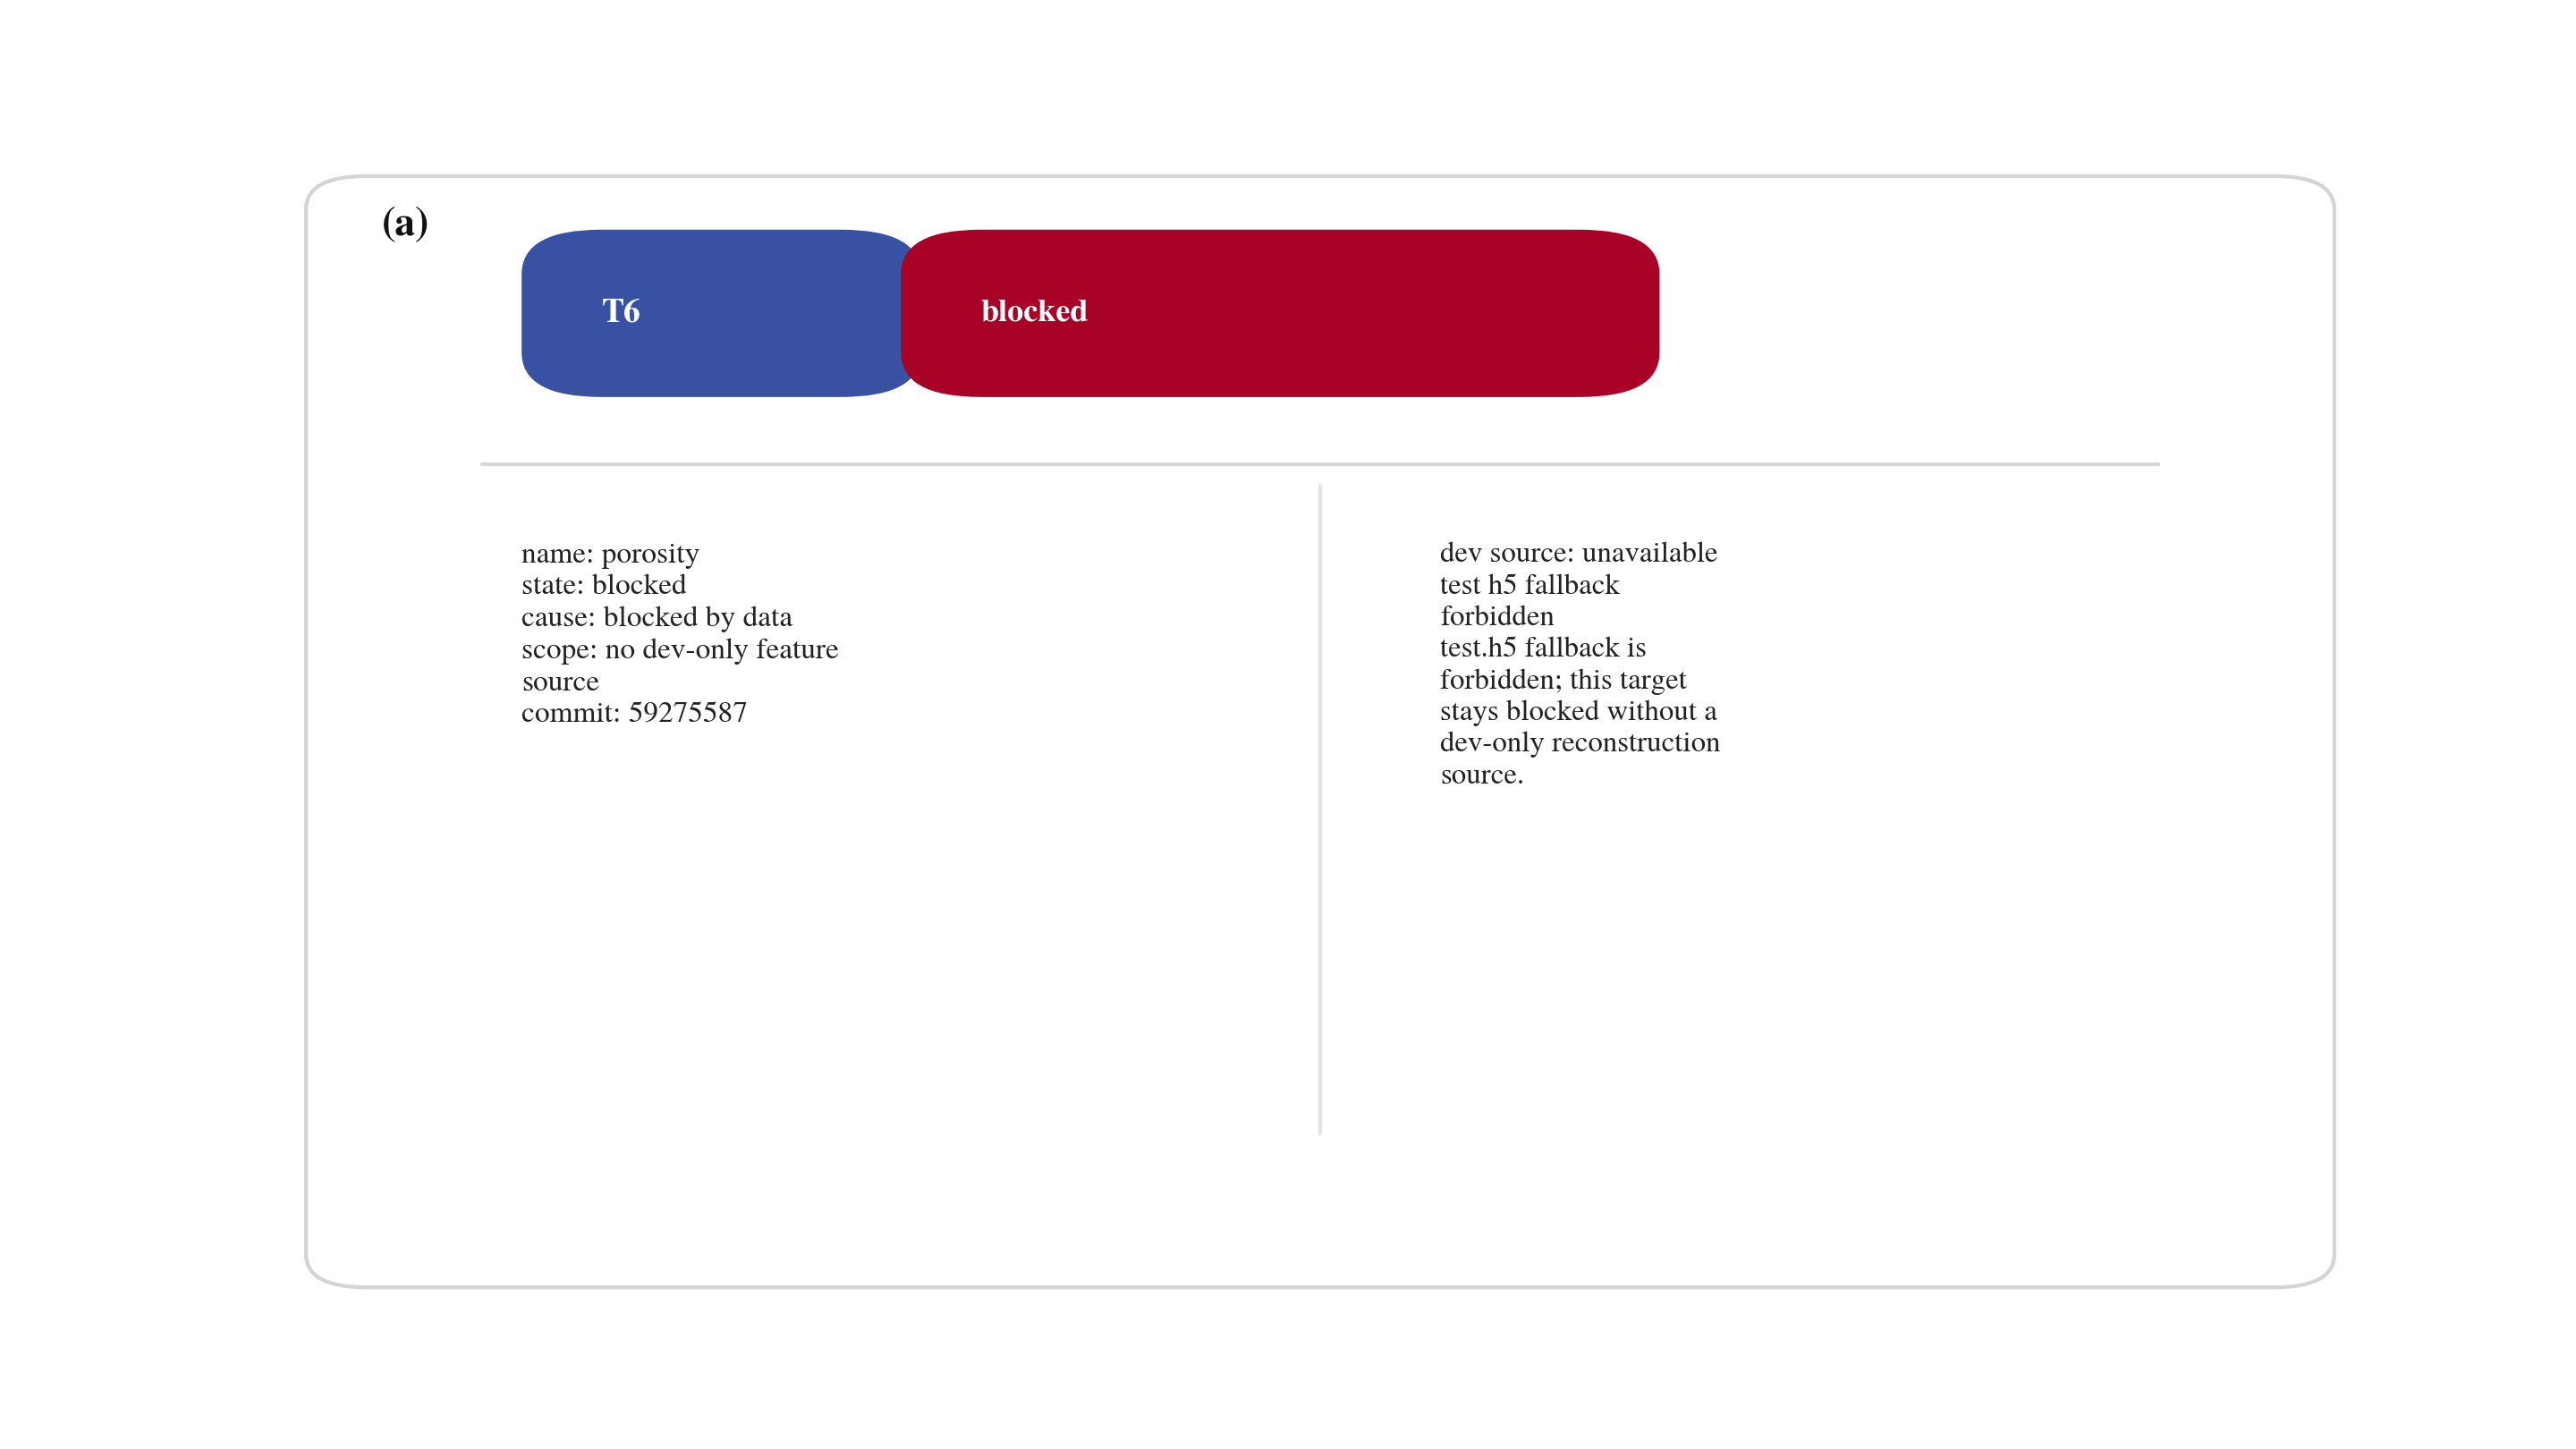
\includegraphics[width=\textwidth]{../figures/results/sweetspot/T6_status_card.png}
    \caption{T6}
  \end{subfigure}\hfill
  \begin{subfigure}[t]{0.32\textwidth}
    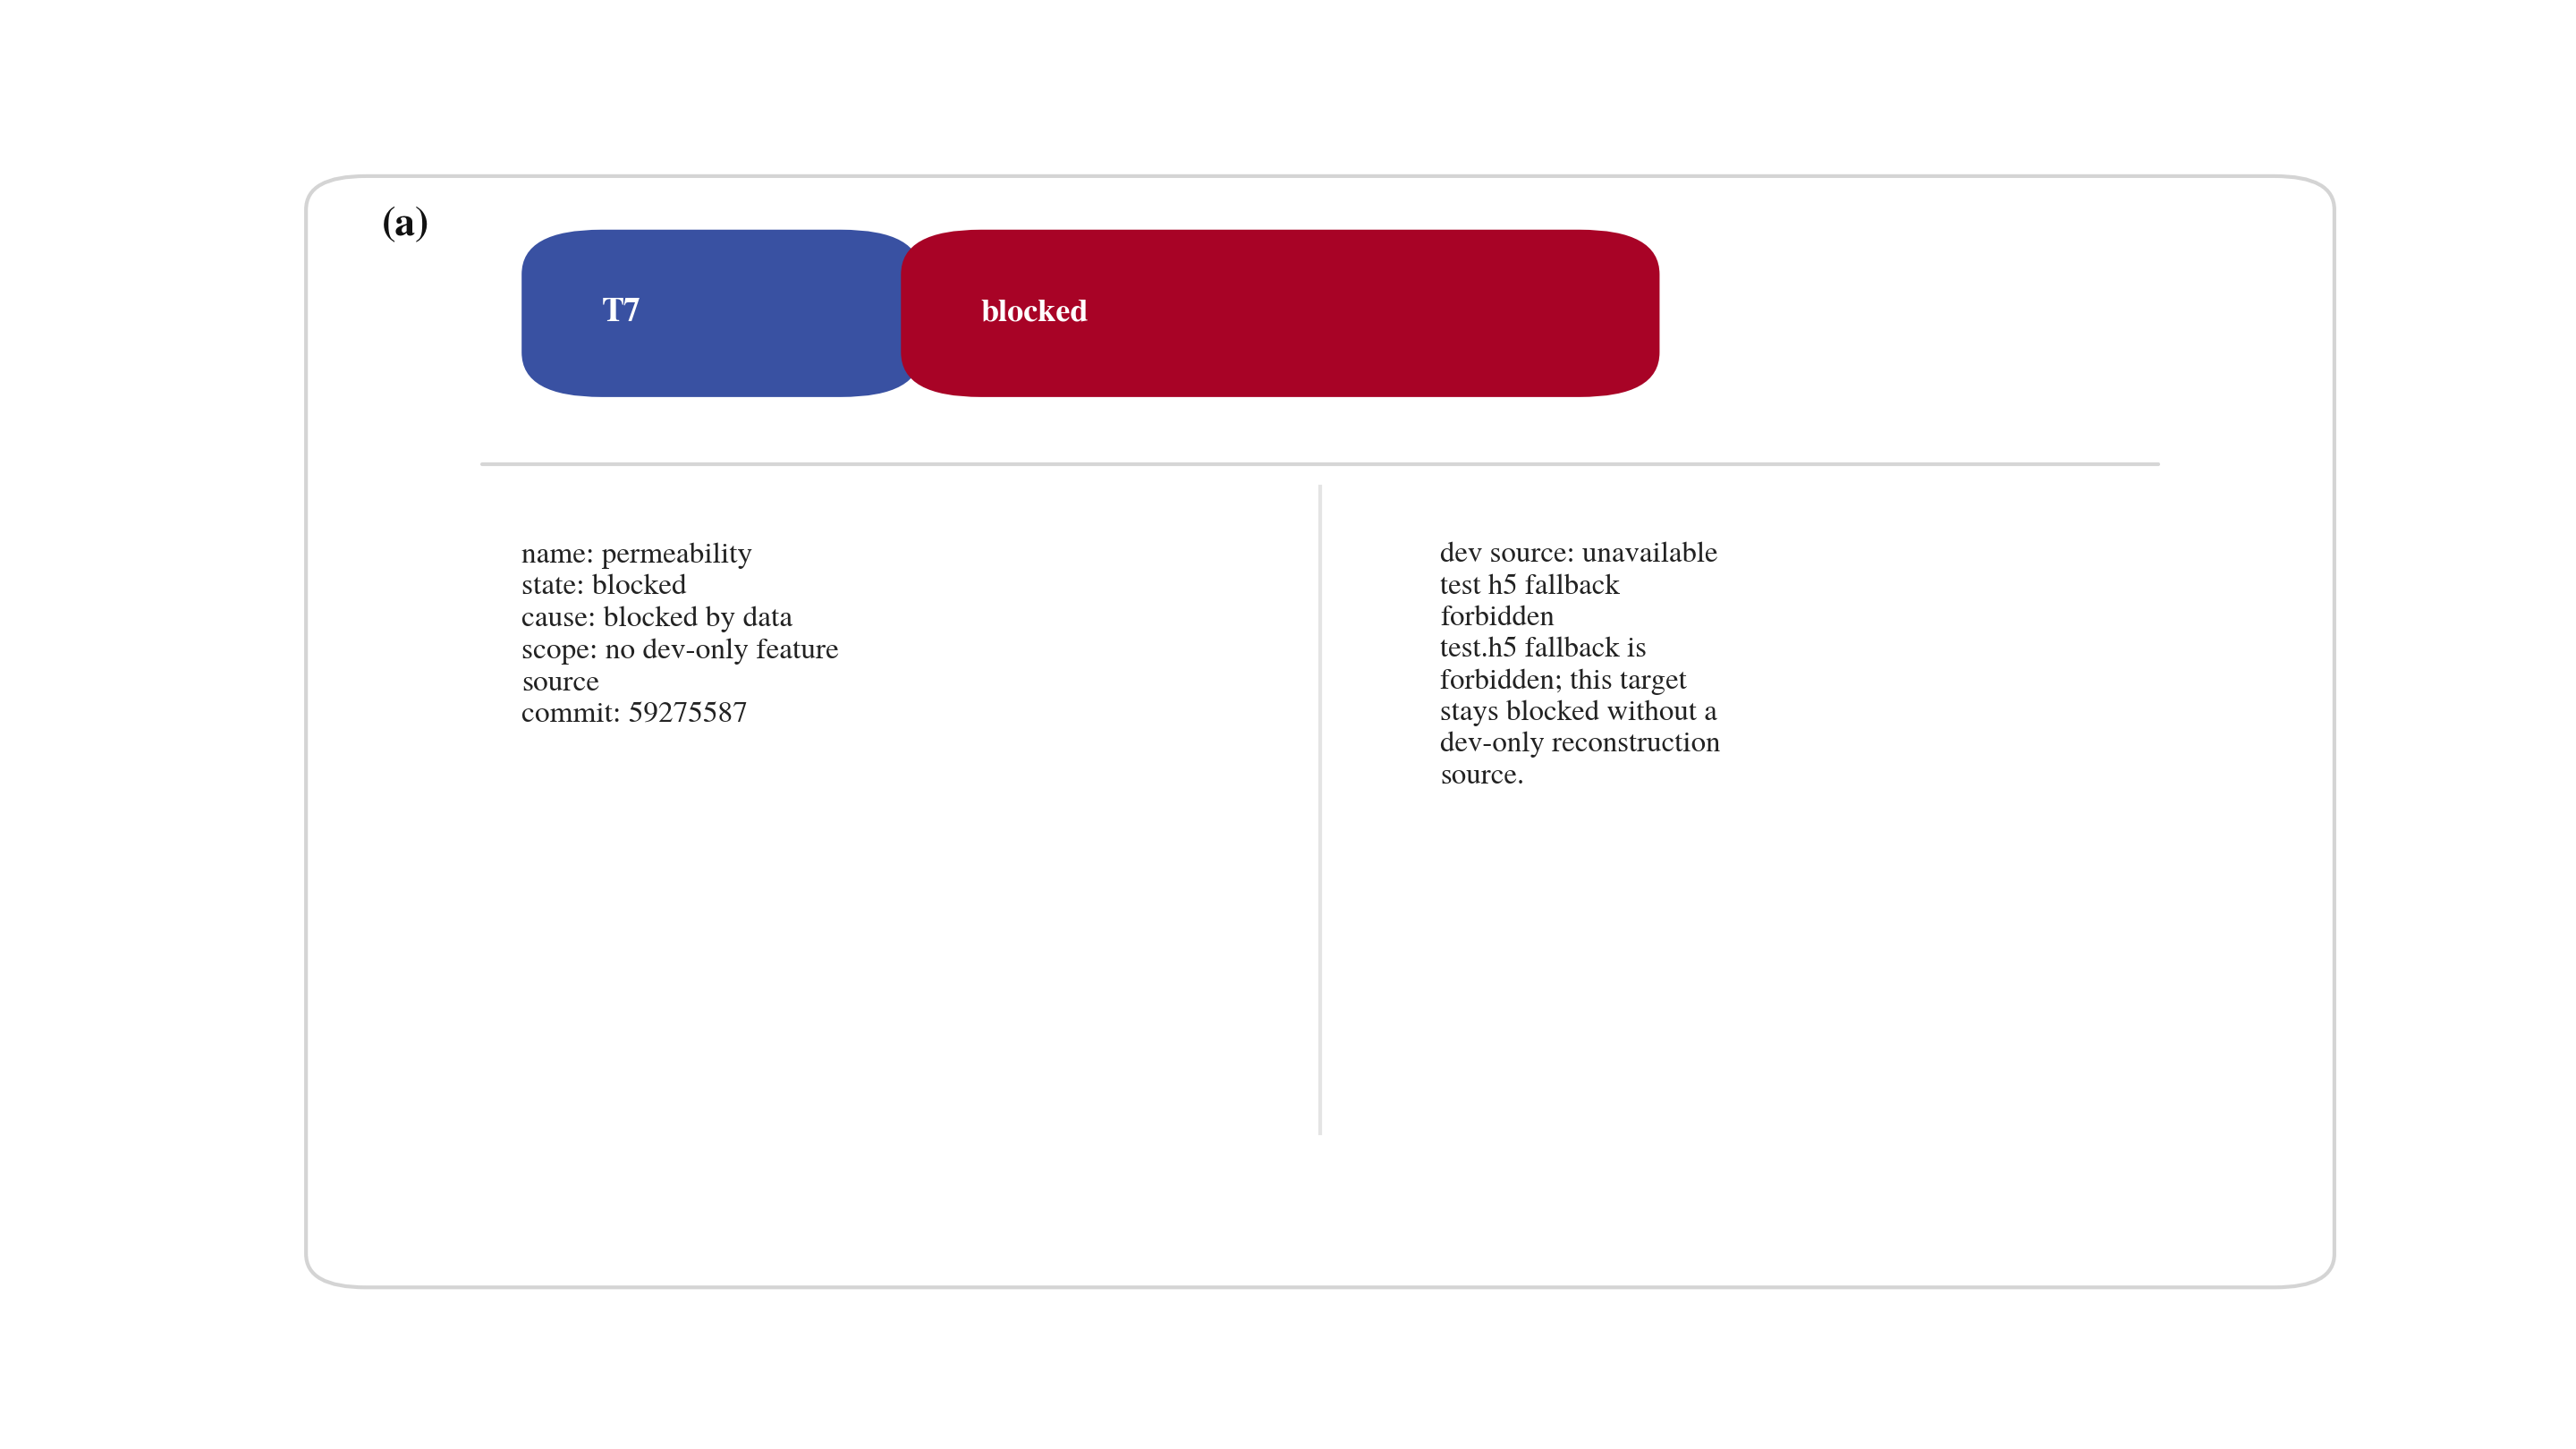
\includegraphics[width=\textwidth]{../figures/results/sweetspot/T7_status_card.png}
    \caption{T7}
  \end{subfigure}
  \caption{T5--T7 的数据可用性。T5 缺少经审定标签，T6--T7 缺少完整多模态开发输入。}
\end{figure}

本次基础模型实验中，明确的开发集改进来自 T3。T1、T2 和 T4 已完成固定模型评价；
T5--T7 在标签或输入不完整时不构造替代结果。逐目标报告避免把不同物理含义和单位的
指标合并为一个表面精确、实际难以解释的综合分数。

\FloatBarrier

\chapter{三维重建}

\section{任务背景}

三维重建根据稀疏井点恢复连续储层属性体。输入包括观测位置
$\{\bm{s}_i\}_{i=1}^{N}$、孔隙度标签 $\{z_i\}_{i=1}^{N}$ 以及与井点配准的
三维地震体，输出为规则网格任意位置 $\bm{s}_0$ 的孔隙度估计。该问题具有明显的
欠定性：井点能够约束局部数值，却不足以单独确定井间结构；地震体覆盖完整空间，
却与孔隙度之间不存在简单的一一对应关系。

普通克里金能稳定表达距离衰减与空间连续性，是稀疏重建的强基线。OpenMind-MAE
等三维地学基础模型则能从地震块中提取多尺度结构表征。前期实验表明，让大模型直接
预测孔隙度或学习克里金残差，容易重复已有空间信号并放大折间波动。本赛道最终采用
一条更稳健的路径：保留克里金主路，用冻结基础模型表征重新定义邻域，再由固定核
集成补充地震结构信息。

\section{方法原理}

普通克里金以观测值的无偏线性组合估计目标点：
\begin{equation}
  \hat{z}_{\mathrm{OK}}(\bm{s}_0)
  =\sum_{i=1}^{N}\lambda_i z_i,
  \qquad \sum_{i=1}^{N}\lambda_i=1,
\end{equation}
其中权重 $\lambda_i$ 由变异函数和空间几何共同确定。它提供可解释、稳定的低方差
预测，但只在预先给定的坐标度量中寻找邻点。

为引入地震结构，配准的三通道三维块首先通过真实预训练的 OpenMind-MAE
编码器\cite{wald2025openmind}，得到 $96$ 维体素特征 $\bm{U}_i$。编码器参数保持
冻结；标准化与主成分变换只在当前外折训练点拟合：
\begin{equation}
  \bm{u}_i=\operatorname{PCA}\!\left(
  \operatorname{Std}_{\mathcal{T}}(\bm{U}_i)\right).
\end{equation}
对地震属性向量 $\bm{a}_i$，构造三组基础模型引导的邻域度量
\begin{equation}
  \bm{m}_{s}(\bm{s}_i)=
  \left[
    \tilde{x}_i,\ \tilde{y}_i,\ 4\tilde{z}_i,
    \ s\tilde{\bm{a}}_i,\ 0.1\bm{u}_i
  \right],
  \qquad s\in\{0,0.1,0.2\},
  \label{eq:reconstruction-metric}
\end{equation}
其中波浪号表示按训练折统计量归一化，系数 $4$ 表示垂向各向异性，$0.1$ 固定
基础模型表征的尺度。每组度量检索 $64$ 个最近邻，并采用幂指数为 $1.5$ 的反距离核：
\begin{equation}
  k_s(\bm{s}_0)=
  \frac{\sum_{i\in\mathcal{N}_{64}(\bm{s}_0)}
  w_i(\bm{s}_0)z_i}
  {\sum_{i\in\mathcal{N}_{64}(\bm{s}_0)}w_i(\bm{s}_0)},
  \quad
  w_i(\bm{s}_0)=
  \left(\lVert\bm{m}_s(\bm{s}_0)-\bm{m}_s(\bm{s}_i)\rVert_2
  +\varepsilon\right)^{-1.5}.
\end{equation}

最终模型对三组核等权平均，再与普通克里金融合：
\begin{equation}
  \hat{z}_{\mathrm{P21}}(\bm{s}_0)
  =0.25\hat{z}_{\mathrm{OK}}(\bm{s}_0)
  +\frac{0.75}{3}\sum_{s\in\{0,0.1,0.2\}}k_s(\bm{s}_0).
  \label{eq:reconstruction-p21}
\end{equation}
这一定义不包含逐折模型选择，也不在评价数据上调整融合权重。基础模型的作用不是
直接输出属性值，而是把地震结构编码进邻域关系；克里金仍负责维持数值稳定性。

\ArchitectureFigure{reconstruction}
  {三维重建模型架构。冻结的 OpenMind-MAE 表征与坐标、垂向各向异性及地震属性共同定义三组固定邻域核，核均值再与普通克里金融合。}
  {reconstruction-architecture}

\section{训练策略}

开发评价沿用五个空间外折，每折固定使用 $512$ 个训练标签和 $2{,}048$ 个验证点。
所有标准化、PCA 与邻域索引均在当前训练折内建立，验证标签不参与特征变换、参数
搜索或模型选择。OpenMind-MAE 保持冻结，因此本方法的训练实质是训练折内的表征
校准、邻域构建与固定参数执行，而不是端到端更新大模型。

LoRA、Adapter 和分阶段解冻曾作为独立训练路线接受检查。张量尺寸、梯度、参数更新
与损失均为有限值，说明这些模块已经真实接入；其中表现最好的 staged-LoRA-r4
取得 $0.027790$ 的 OOF RMSE，但仍未超过当时的 P19 参考模型 $0.027751$。
因此这些可训练路线保留为诊断实验，默认配置全部关闭；部署路径只启用
\Cref{eq:reconstruction-p21} 的固定 P21 集成。

\TrainingFlow
  {井点与三维地震配准}
  {空间五折划分}
  {冻结基础模型取特征}
  {训练折标准化与 PCA}
  {固定三核集成与融合}
  {三维重建训练与推理流程}
  {reconstruction-training}

\section{实验设计}

实验分为开发评价与迁移压力测试。开发评价在同一组五个空间折上比较普通克里金、
经去重修正的 P19 基础模型邻域、P20 staged-LoRA-r4 和最终 P21 固定三核集成。
该阶段回答两个问题：地学基础模型表征能否改善邻域检索，以及取消逐折元选择后能否
维持或改善性能。

迁移压力测试在读取目标指标前完成预注册，锁定数据来源、空间映射、五折划分、
PyKrige 1.7.3 基线、P21 参数与成功门槛。测试目标为同一 Volve 场区中此前未被
现有管线使用的历史孔隙度属性版本；开指标后没有重新调参。输入几何、地震表征和
标签预算保持不变，只替换目标属性版本，从而检验固定邻域度量是否依赖某一个开发
目标。该测试属于同场区历史版本迁移，不是跨场区验证、赛事隐藏测试或首次盲测。

\section{评估指标}

三维重建使用 RMSE、MAE 和 Bias：
\begin{align}
  \Metric{RMSE} &= \sqrt{\frac{1}{N}\sum_i(z_i-\hat{z}_i)^2},\\
  \Metric{MAE} &= \frac{1}{N}\sum_i|z_i-\hat{z}_i|,\\
  \Metric{Bias} &= \frac{1}{N}\sum_i(\hat{z}_i-z_i).
\end{align}
RMSE 为主指标，MAE 衡量典型绝对误差，Bias 检查整体偏移。开发阶段同时报告相对
P19 的折级胜、平、负与整折 bootstrap；历史版本测试的预注册门槛为相对 PyKrige
的 pooled RMSE 改善不少于 $1\%$，且五个空间折中最多一折退步。置信区间用于说明
不确定性，不在开指标后改写成功门槛。

\section{实验结果}

\begin{table}[htbp]
  \centering
  \caption{三维重建开发空间折的主要结果}
  \label{tab:reconstruction-development}
  \begin{tabular}{lrrl}
    \toprule
    模型 & RMSE & MAE & 研究角色 \\
    \midrule
    普通克里金 & 0.028450 & 0.021413 & 基线 \\
    P19 基础模型邻域 & 0.027751 & 0.020826 & 参考模型 \\
    P20 staged-LoRA-r4 & 0.027790 & 0.020871 & 未采用 \\
    P21 固定三核集成 & \textbf{0.027734} & \textbf{0.020799} & 最终模型 \\
    \bottomrule
  \end{tabular}
\end{table}

P21 相对普通克里金的开发 OOF RMSE 降低 $2.5144\%$，相对 P19 再降低
$0.0613\%$。与 P19 比较时，一折改善、四折数值等价、没有折退步。整折
bootstrap 给出的候选更优概率为 $0.70075$，RMSE 差值的 $95\%$ 区间为
$[-6.50\times10^{-5},0]$。因此 P21 被接受为更简单的确定性改进，但不据此声称
广泛统计效应，也不把全部增益归因于某一单独组件。

\begin{table}[htbp]
  \centering
  \caption{冻结 P21 的同场区历史版本迁移结果}
  \label{tab:reconstruction-transfer}
  \begin{tabular}{lrrrl}
    \toprule
    模型 & RMSE & MAE & Bias & 空间折 \\
    \midrule
    普通克里金 & 0.028235 & 0.021294 & -0.001011 & -- \\
    冻结 P21 & \textbf{0.027825} & \textbf{0.020826} & 0.000513 & 4 胜 1 负 \\
    \bottomrule
  \end{tabular}
\end{table}

在未用于开发的历史属性版本上，冻结 P21 的 RMSE 相对 PyKrige 降低
$1.4529\%$，通过预注册门槛；整折 bootstrap 的候选更优概率为 $0.94595$，
$95\%$ 差值区间为 $[-9.16\times10^{-4},8.81\times10^{-5}]$，仍跨越零。
该结果表明，大模型表征进入固定邻域度量后能够在目标版本变化下保留增益，但证据
范围仍限于同一场区。

\ResultFigure{0.94}{reconstruction}{before_after_primary_metric.png}
  {三维重建的开发空间折与历史版本迁移结果。两个面板使用不同目标版本，数值只在面板内比较。}

\ResultFigure{0.99}{reconstruction}{research_native_volume.png}
  {Volve MAPAXES 配准网格中的参考孔隙度、条件留出真值、重建结果和“预测减真值”残差。残差表示已知留出点上的观测误差，不是不确定性预测。}

\ResultFigure{0.94}{reconstruction}{research_orthogonal_diagnostics.png}
  {条件留出网格的三组正交切片。三行依次为真值、重建和残差，三列为 K、J 和 I 法向切面。}

\ResultFigure{0.92}{reconstruction}{research_directional_variogram.png}
  {条件留出网格的方向经验变差函数。左图沿 K 索引方向，右图合并 I--J 索引方向；横轴距离由 MAPAXES 坐标计算。}

这些三维图件用于检查属性范围、切片连续性与方向空间相关，不替代上述空间折指标。
现有条件重建仍表现出细尺度方差不足，说明点值 RMSE 改善并不等于全部地质结构已经
恢复。当前默认配置因此冻结 P21，关闭未晋级的 LoRA、Adapter、分阶段解冻与残差
旁路。本报告以同场区历史版本迁移作为当前验证终点，不再围绕同一目标版本调参，
也不追加跨数据集测试；后续若获得独立新井，可将其作为新的外部证据，而不回写本次
模型选择。

\FloatBarrier

\chapter{总结展望}

本报告以统一结构比较了六个地学智能赛道。结果显示，模型选择必须服从任务的数据
形态和样本规模。树模型在储层物性与岩相任务中仍具有稳定优势；SAM2 交叉注意力和
Chronos-2 分别在地震相与 T3 开发实验中取得改进。三维重建则通过改变基础模型的
接入位置取得进展：冻结 OpenMind-MAE 表征不再直接回归孔隙度，而是参与邻域度量，
固定三核集成在开发空间折和同场区历史版本迁移中均低于 PyKrige 的 RMSE。

新增空间诊断进一步说明，点值指标并不足以支撑地学模型。断层结果需要回到地震剖面
核对几何位置，多个物性目标需要检查联合关系，生产预测需要检查时序残差，三维重建
还必须评价方向空间相关。P21 改善了点值误差，但现有条件重建的方向变差仍小于真值；
这两项观察并不冲突，它们分别描述数值预测和细尺度空间结构。

\begin{table}[htbp]
  \centering
  \caption{六个赛道的主要结果与后续实验}
  \label{tab:conclusion}
  \small
  \begin{tabularx}{\textwidth}{>{\raggedright\arraybackslash}p{2.50cm}YY}
    \toprule
    赛道 & 主要结果 & 后续实验 \\
    \midrule
    断层预测 & 二维基线高召回、低精确率 & 建立连续三维开发折 \\
    地震相分割 & 开发集 mIoU 提高 0.1160 & 补同架构随机初始化对照 \\
    储层物性预测 & 树模型留出 $R^2$ 为 0.8891--0.9807 & 校准长尾区间并补新井族 \\
    岩相分类 & MOMENT 略优于随机初始化但弱于 XGBoost & 扩大母井与少数类样本 \\
    甜点评价 & T3 开发 MAE 为 186.57 & 完成同口径留出评价 \\
    三维重建 & P21 开发 RMSE 为 0.027734，历史版本迁移改善 1.4529\% & 冻结 P21，继续检查细尺度空间结构 \\
    \bottomrule
  \end{tabularx}
\end{table}

后续有三项优先工作。第一，为断层预测建立合法的三维开发折，使 SAM-Med3D
候选模型具备公平评价条件。第二，为地震相基础模型分支补充同架构随机权重对照，
并为 Chronos-2 完成同口径时序留出评价；岩相分类已完成预训练归因，应转向扩大
数据与改善少数类学习。第三，冻结三维重建的 P21 默认配置，不再扩展未晋级的
LoRA、Adapter 或残差旁路。当前报告不追加跨数据集测试，后续工作转向检查细尺度
空间结构和不确定性。若未来获得独立新井，再将其作为额外验证，而不回写本次模型选择。

报告结构已经为后续实验预留扩展空间。新增模型时，应在对应赛道的“方法原理”和
“训练策略”中说明变化。新增数据或对照时，应更新“实验设计”。新增结果则进入
“实验结果”，并保持原有指标口径。这样可以持续扩充内容，而不破坏六赛道之间的
可比性。


\appendix
\chapter{复现说明}

\section{文档真源}

报告的 LaTeX 真源、编译入口和图件目录分别为：
\begin{itemize}
  \item \path{_paper/technical_report/src/}
  \item \path{_paper/technical_report/build_report.sh}
  \item \path{_paper/technical_report/figures/}
\end{itemize}

各赛道的定量结论来自已归档的 JSON 指标文件。模型、图件与来源之间的对应关系记录在
\path{_paper/technical_report/report_manifest.yml}。后续扩展应先更新赛道实验，
再更新清单与正文，避免手工改写数值造成不一致。

\section{图件生成}

模型架构图采用 Nano Banana 2 生成。初版与审阅修订提示词分别保存在：
\begin{itemize}
  \item \path{_paper/technical_report/prompts/nano_banana_v1/}
  \item \path{_paper/technical_report/prompts/nano_banana_v2/}
  \item \path{_paper/technical_report/prompts/nano_banana_v3/} 至
        \path{_paper/technical_report/prompts/nano_banana_v5/}
\end{itemize}
架构图用于解释信息流，不作为模型性能证据。数据图由下列流水线统一生成：
\begin{itemize}
  \item \path{_pipelines/05_research_visualization_expansion/}
\end{itemize}
真实输入、证据类型、图片尺寸和哈希记录在：
\begin{itemize}
  \item \path{_outputs/research_visualization_expansion/v1/artifact_manifest.json}
\end{itemize}
正文只引用已经人工检查的成品。

基础模型的强基线、随机初始化、预训练初始化和融合条件记录在
\path{_pipelines/05_research_visualization_expansion/foundation_model_experiment_contract.json}。
该合同约束后续实验的可比性，不把待完成实验写成既有结果。

\section{扩展方式}

后续版本可以增加新模型、消融实验、计算开销和新盲测，但六个赛道的固定六节目录
保持不变。新增结果应同时保存数据划分、参数、随机种子、指标文件和图件；若评价集
已经被用于模型选择，必须在正文中继续标明为已知留出集。


\renewcommand{\bibname}{参考文献}
\bibliographystyle{unsrtnat}
\bibliography{references}

\end{document}
